\documentclass[10pt,journal,compsoc,draftclsnofoot]{IEEEtran}

\makeatletter    
    \if@compatibility
\renewenvironment{titlepage}
    {%
      \cleardoublepage
      \if@twocolumn
        \@restonecoltrue\onecolumn
      \else
        \@restonecolfalse\newpage
      \fi
      \thispagestyle{empty}%
      %\setcounter{page}\z@
    }%
    {\if@restonecol\twocolumn \else \newpage \fi
    }
\else
\renewenvironment{titlepage}
    {%
      \cleardoublepage
      \if@twocolumn
        \@restonecoltrue\onecolumn
      \else
        \@restonecolfalse\newpage
      \fi
      \thispagestyle{empty}%
      %\setcounter{page}\@ne
    }%
    {\if@restonecol\twocolumn \else \newpage \fi
     \if@twoside\else
       % \setcounter{page}\@ne
     \fi
    }
\fi
\makeatother

% Definition of \subparagraph
\makeatletter
\newcommand\subparagraph{%
  \@startsection{subparagraph}{5}
  {\parindent}
  {3.25ex \@plus 1ex \@minus .2ex}
  {0.75ex plus 0.1ex}
  {\normalfont\normalsize\bfseries}}
\makeatother

\makeatletter
\newcommand\subsubparagraph{%
  \@startsection{subsubparagraph}{6}
  {\parindent}
  {3.25ex \@plus 1ex \@minus .2ex}
  {0.75ex plus 0.1ex}
  {\normalfont\normalsize\bfseries}}
\makeatother

\newcounter{subparagraph}[paragraph]
\newcounter{subsubparagraph}[subparagraph]

\makeatletter
\def\toclevel@subsubparagraph{6}
\makeatother

\usepackage{listings}
\usepackage{color}
\usepackage{titlesec}
\usepackage{float}
\usepackage{hyperref}
\usepackage{array}
\usepackage{tocloft}
\usepackage{lscape}
\usepackage{textcomp}
\usepackage{pgfgantt}
\usepackage{amsmath}
\usepackage{lipsum}
\usepackage{setspace}
\usepackage{pdfpages}

\usepackage{geometry}
\geometry{margin=0.75in}

\setcounter{tocdepth}{2}
\setcounter{secnumdepth}{4}

\definecolor{codegreen}{rgb}{0,0.6,0}
\definecolor{codegray}{rgb}{0.5,0.5,0.5}
\definecolor{codepurple}{rgb}{0.58,0,0.82}
\definecolor{backcolour}{rgb}{0.95,0.95,0.92}
\definecolor{light-gray}{gray}{0.95}

\lstdefinestyle{mystyle}{
    backgroundcolor=\color{backcolour},   
    commentstyle=\color{codegreen},
    keywordstyle=\color{magenta},
    numberstyle=\tiny\color{codegray},
    stringstyle=\color{codepurple},
    basicstyle=\footnotesize,
    breakatwhitespace=false,         
    breaklines=true,                 
    captionpos=b,                    
    keepspaces=true,                             
    numbersep=5pt,                  
    showspaces=false,                
    showstringspaces=false,
    showtabs=false,                  
    tabsize=2
}

\lstset{style=mystyle}

\begin{document}
\onecolumn

\begin{titlepage}
\null
\vspace{15mm}

\begin{flushleft}
\begin{bfseries}
	\vskip2mm
	\Huge{Final Report for\\ Better Graphics For A Robotics Grasping GUI}\\
	\vspace{15mm}
	\textbf{\huge Shady Robots} \\
	\vskip2mm
	\large{Group 12}
	\vskip5mm
	\Large{Justin Bibler \\
	Matthew Huang \\
	Daniel Goh \\}
\end{bfseries}

\vspace{15mm}
\Large{CS463: Senior Software Engineering Project} \\
\Large{Spring 2017} \\

\vspace{5mm}

\today

\vfill

\begin{normalsize}
{\bf Abstract:}
This document goes over the project's background, requirements, designs used, technology review, weekly team updates, final poster, documentation, useful resources, and project prospect for the team members.

{\bf Keywords:} OpenRAVE, shaders, warm cool shading, silhouettes, shadows, robotic simulation, geometry, visualization, render, ubuntu, vmware, virtualbox
\end{normalsize}
\end{flushleft}

\newpage

\end{titlepage}

\begin{flushleft}

\tableofcontents

\newpage

\section{Introduction}
Better Graphics For A Robotics Grasping GUI was requested by Cindy Grimm.
This project was requested to improve the robotics simulation's (OpenRAVE) graphics, which its visuals are used in a user study that she is involved in.
The team that worked on this project was Shady Robots, which consists of Justin Bibler, Matthew Huang, and Daniel Goh.
Justin Bibler and Matthew Huang were responsible for the technical implementations.
This include implementing warm cool shading, shadows, and silhouettes in OpenRAVE.
Daniel Goh was responsible for the non-technical aspects of the project, which include communication, documentation, and capstone-related deliverables.
Cindy Grimm was our advisor throughout the project, providing supervision and advice throughout the term. 
\newpage

\section{Requirements Document}

Refer to next page for the initial requirements document.

\newpage

\onecolumn

\begin{titlepage}
\null
\vspace{35mm}

\begin{flushleft}
\begin{bfseries}
	\vskip2mm
	\Huge{Requirements Document for\\ Better Graphics For A Robotics Grasping GUI}\\
	\vspace{30mm}
	\textbf{\huge Shady Robots} \\
	
\end{bfseries}

\vspace{15mm}
\Large{CS461: Senior Software Engineering Project} \\
\Large{Fall 2016} \\

\vspace{10mm}

\today

\end{flushleft}

\newpage
\null
\vspace{35mm}

\begin{flushleft}
\begin{bfseries}
	\vskip2mm
	\Huge{Requirements Document for\\ Better Graphics For A Robotics Grasping GUI}\\
	\vspace{30mm}
	\textbf{\huge Shady Robots} \\
	
\end{bfseries}

\vspace{15mm}
\Large{CS461: Senior Software Engineering Project} \\
\Large{Fall 2016} \\

\vspace{10mm}

\today

\vfill

\begin{normalsize}
{\bf Abstract:}
Our customer is using a simulation to create visuals that are used for online data collection.
This simulation is using outdated libraries which result in outdated graphics.
We, as the supplier define the requirements necessary to accomplish our customer's request.
The request being to update the simulation's graphics with warm cool shaders, shadows and silhouettes.

{\bf Keywords:} OpenInventor, OpenGL, OpenRave, shaders, warm cool shaders, silhouettes, shadows, robotic simulation, geometry, visualization, render,
vertex lines, software requirements specification, system requirements specifications
\end{normalsize}
\end{flushleft}

\newpage

\end{titlepage}

\subsection{Introduction}
\vspace{3mm}
Currently, our client is using visualizations, of a robot hand grasping objects, to collect data online.
These visualizations are created from a simulation program (OpenRave), the data collected is used to create a model of the human grasp.
However, the current graphics in the simulation are outdated.
It is hard to see and understand the shapes and contact points represented in the scene.
Because of this, users aren't confident in giving proper responses to the simulation.
Thus, the graphics need to be updated to allow meaningful data to be collected. \\


\subsection{Participants}
\vspace{3mm}
Cindy Grimm, Matthew Huang, Daniel Goh and Justin Bibler \\ 

\newpage

\newpage
\begin{flushleft}
\subsection{Overview}
\vspace{3mm}
This document describes requirements needed to enhance the current OpenRave simulation. 
Clause 2 lists the references made to other documents. 
Clause 3 provides definitions of specific terms used.
Clause 4 lists the specific requirements that will be met.
This includes the external interface requirements, functional requirements, performance requirements, design constraints, software system attributes, and other requirements.

\subsection{References}
\vspace{3mm}

Gooch Shading \footnote{\label{note1}ECGLAB. Gooch Shading. Retrieved from: https://lva.cg.tuwien.ac.at/ecg/wiki/doku.php?id=students:gooch}
\vspace{3mm}

IEEE Std 830-1998, IEEE Recommended Practice for Software Requirements Specifications \footnote{\label{note2}IEEE publications are available from the Institute of Electrical and Electronics Engineers, 445 Hoes Lane, P.O. Box 1331, Piscataway, NJ 08855-1331, USA.}
\vspace{3mm}

Shadow Mapping \footnote{\label{note3} Shadow Mapping. LearnOpenGL. Retrieved from: http://learnopengl.com/\#!Advanced-Lighting/Shadows/Shadow-Mapping}
\vspace{3mm}

Silhouette Extraction \footnote{\label{note4}Gooch, Bruce. Silhouette Extraction. Retrieved from: http://www.cs.rutgers.edu/~decarlo/readings/gooch-sg03c.pdf}

\subsection{Definitions}

\vspace{3mm}
\textbf{Contract:}
A legally binding document agreed upon by the customer and supplier. This includes the technical and organizational requirements, cost, and schedule for a product. A contract may also contain informal but useful information such as the commitments or expectations of the parties involved.

\vspace{3mm}
\textbf{Customer:}
The person, or persons, who pay for the product and usually (but not necessarily) decide the requirements. In the context of this recommended practice the customer and the supplier may be members of the same organization.

\vspace{3mm}
\textbf{Supplier:}
The person, or persons, who produce a product for a customer.

\vspace{3mm}
\textbf{User:}
The person, or persons, who operate or interact directly with the product. The user(s) and the customer(s) are often not the same person(s).

\vspace{3mm}
\textbf{Modern Computer:}
Modern computer defined by the Oregon State University (OSU) EECS minimum laptop requirements: 
Intel Core i5 or i7, or AMD A8 and AMD A10 APU 8GB RAM

\newpage

\subsection{Specific requirements}
\vspace{3mm}

\subsubsection{External interface requirements}
\vspace{3mm}
The purpose of the software's output is to give a visual understanding of the robot's grasping capabilities.
The software will accept an input simulation file (.py file) through the console.
The software will then output a simulation onto a new window.

\subsubsection{Functional requirements}
\vspace{3mm}
The system shall render the scene and output to a new window.
The rendered scene shall include all 3D objects to be displayed in the scene with correct geometry.
No objects should have clashing vertex lines, and all shapes should be drawn as intended by the user.
Refer to Fig. 1 below.

\begin{figure} [h]
  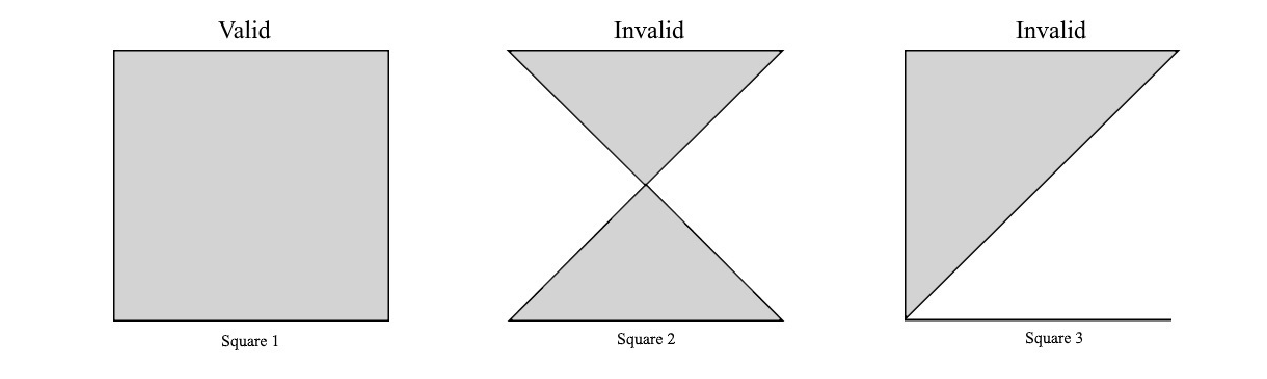
\includegraphics[width=\linewidth]{reqdoc_v1/squares.eps}
  \caption
{ \newline \hspace{\linewidth}
Square 1: Vertex lines drawn correctly resulting in desired geometry. \newline \hspace{\linewidth}
Square 2: Vertex lines cross resulting in undesired geometry. \newline \hspace{\linewidth}
Square 3: Incorrect vertex line drawing resulting in undesired geometry.}
  \label{fig:squares}
\end{figure}

\vspace{3mm}

The scene shall include:
\paragraph{Warm cool shaders}
Refer to "Description" section of Gooch Shading listed in this document's references section.

\paragraph{Shadows}
A dark area or shape produced by a body coming between rays of light and a surface.

\paragraph{Silhouettes}
Refer to "Definition of a Silhouette" section of Silhouette Extraction listed in this document's references section.

\vspace{3mm}
The system shall continuously re-render the scene until completion of the simulation or software termination.

\subsubsection{Performance requirements}
\vspace{3mm}
\begin{itemize}
\item The system output should maintain a minimum stable 30FPS on an average modern computer.
\begin{itemize}
\item Modern computer defined by the Oregon State University (OSU) EECS minimum laptop requirements: \\
Intel Core i5 or i7, or AMD A8 and AMD A10 APU
8GB RAM

\end{itemize}
\item The system will only run one simulation per window.
\item The initial scene will be rendered within the first 30 seconds after accepting an input file.
\end{itemize}

\subsubsection{Design constraints}
\vspace{3mm}
\begin{itemize}
\item The system currently utilizes outdated OpenGL libraries.
\item The location of the main render loop is not known to the customer.
\item OpenRave is not open sourced.
\end{itemize}


\subsubsection{Software system attributes}
\vspace{3mm}
\paragraph{Reliability}
\vspace{5mm}
The system shall always run properly created simulations.


\paragraph{Maintainability}
\vspace{3mm}
The system shall:
\begin{itemize}
\item Be easily maintained and upgraded. 
\item Have well documented and easily testable functions.
\item Have functions with single, clear purposes; they should not overlap in what they do.
\end{itemize}

\paragraph{Portability}
\vspace{3mm}
The system shall work on Linux operating systems.

\subsubsection{Other requirements}
\vspace{3mm}
The outdated OpenGL libraries will be updated to utilize OpenGL 3.0 libraries.

\vfill

\newpage

\begin{landscape}
\subsection{Gantt Chart}
\vfill
\begin{ganttchart}[hgrid, vgrid={{draw=none}, dotted}]{1}{36}
\gantttitle{Fall 2016}{12} 
\gantttitle{Winter 2017}{12}
\gantttitle{Spring 2017}{12} \\
\gantttitlelist{1,...,12}{1} 
\gantttitlelist{1,...,12}{1}
\gantttitlelist{1,...,12}{1} \\
\ganttbar{Familiarize Project}{1}{8} \\
\ganttbar{Identify render loop}{9}{16} \\ 
\ganttbar{Implement warm cool shaders in simulation}{9}{16} \\ 
\ganttmilestone{Warm Cool Shaders Implementation Milestone}{16} \\
\ganttbar{Implement silhouettes in simulation}{9}{16} \\
\ganttmilestone{Silhouettes Implementation Milestone}{16} \\
\ganttbar{Switch to 2-pass rendering}{17}{22} \\ 
\ganttbar{Implement shadows in simulation}{17}{22} \\ 
\ganttmilestone{Shadows Implementation Milestone}{22} \\
\ganttbar{Aesthetic evaluation and maintenance}{23}{26} \\
\ganttbar{Conduct user interviews}{25}{30} \\
\ganttbar{Finalize and prepare for expo}{29}{34} \\
\end{ganttchart}
\newline
\begin{center}
Gantt Chart for Shady Robots' Senior Design Project
\end{center}
\vfill
\end{landscape}

\newpage

\null
\vfill

\noindent\begin{tabular}{ll}
\makebox[2.5in]{\hrulefill} & \makebox[2.5in]{\hrulefill}\\
Cindy Grimm & Date\\[4ex]% adds space between the signatures
\makebox[2.5in]{\hrulefill} & \makebox[2.5in]{\hrulefill}\\
Justin Bibler & Date\\[4ex]% adds space between the signatures
\makebox[2.5in]{\hrulefill} & \makebox[2.5in]{\hrulefill}\\
Matthew Huang & Date\\[4ex]% adds space between the signatures
\makebox[2.5in]{\hrulefill} & \makebox[2.5in]{\hrulefill}\\
Daniel Goh & Date\\
\end{tabular}

\end{flushleft}

\section{Requirements Document Update}

\begin{center}
\begin{table}[H]
\caption{Table showing the requirement that is changed (Requirement), what happened to it (Change Details), and comments for the change(Comments).}
\begin{tabular}{ | p{0.3\linewidth} | p{0.3\linewidth} | p{0.3\linewidth} | }
\hline
\textbf{Requirement}  & \textbf{Change Details}  & \textbf{Comments} \\ \hline

Warm Cool Shading. & 
None. & 
Requirement did not change. \\ \hline

Silhouettes. & 
None. & 
Requirement did not change. \\ \hline

Shadows. & 
None. & 
Requirement did not change. \\ \hline

Initial render must be done within 30s. & 
None. & 
Requirement did not change. \\ \hline

Scene must run at a constant 30 fps. & 
Removed. & 
Requirement was not necessary for the client's purposes. \\ \hline

The system will work on an average modern computer. &
None. &
Requirement did not change. \\ \hline

The system will only run one simulation per window. &
None. &
Requirement did not change \\ \hline

The system shall run properly created simulations. &
None. &
This means that the system will always run valid environment files. \\ \hline

System shall be easily maintained and upgraded.
Have well documented and easily testable functions.
Have functions with single, clear purposes. &
None. &
After speaking with Mike Bailey we discovered that testing graphics is primarily done be ensuring that separate computers create the same render. 
Opposed to unit testing which is very difficult and only analyzes fragment positions.
This process can be done by rendering the scene and examining it. 
In our implementations we have minimal amount of new functions.
This is because most of the work done was hacked into the initializations and uses built in coin3d modules. \\ \hline

The system shall continuously re-render the scene until completion of the simulation or software termination. &
None. &
Requirement did not change. \\ \hline

The system shall work on Linux operating systems. &
None. &
Operating systems became limited due to Openrave.
Our current implementation does work on Linux, within Ubuntu 16.04. \\ \hline

Outdated OpenGL libraries will be updated to utilize OpenGL 3.0 libraries. &
None. &
We were unable to directly import new libraries as this was abstracted out from us.
However, we did update the environment that was given to us to Ubuntu 16.04 which utilizes OpenGL 3.0 while rendering. \\ \hline

\end{tabular}
\newline
\label{table:RequirementsDocumentUpdate}
\end{table}
\end{center}

The original Gantt chart was not modified.

\newpage

\section{Design Document}

Refer to next page for the initial design document.

\newpage

\onecolumn

\begin{titlepage}
\null
\vspace{15mm}

\begin{flushleft}
\begin{bfseries}
	\vskip2mm
	\Huge{Design Document for\\ Better Graphics For A Robotics Grasping GUI}\\
	\vspace{15mm}
	\textbf{\huge Shady Robots} \\
	\vskip2mm
	\large{Group 12}
	\vskip5mm
	\Large{Justin Bibler \\
	Matthew Huang \\
	Daniel Goh \\}
\end{bfseries}

\vspace{15mm}
\Large{CS461: Senior Software Engineering Project} \\
\Large{Fall 2016} \\

\vspace{5mm}

\today

\vfill

\begin{normalsize}
{\bf Abstract:}
Our customer is using a simulation to create visuals that are used for online data collection.
This simulation is using outdated libraries which result in outdated graphics.
Design definitions outlined in this document will be used to accomplish our customer's request.
The request being to update the simulation's graphics with warm cool shaders, shadows and silhouettes.

{\bf Keywords:} OpenInventor, OpenGL, OpenRave, shaders, warm cool shaders, silhouettes, shadows, robotic simulation, geometry, visualization, render, vertex lines
\end{normalsize}
\end{flushleft}

\newpage

\end{titlepage}

\subsection{Introduction}
\begin{flushleft}

\subsubsection{Purpose}
The purpose of this document is to elaborate on the design and logic of how we will be implementing our requirements.

\subsubsection{Scope}
The scope of this document is solely about how new features will be implemented and how those implementations will be tested.

\subsubsection{Context}
Currently, our client is using visualizations, of a robot hand grasping objects, to collect data online.
These visualizations are created from a simulation program (OpenRave); the data collected is used to create a model of the human grasp.
However, the current graphics in the simulation are outdated.
It is hard to see and understand the shapes and contact points represented in the scene.

The context of this document is focused primarily on the visuals of the project.

\subsubsection{Summary}
In clauses 3 to 5, Matthew Huang outlines the design of Gooch shading, silhouettes, and run-time analysis with CodeXL respectively.
In clauses 6 to 8, Justin Bibler outlines the design of shadow volumes, performance benchmarks using FRAPS \cite{fraps}, and methods of code maintainability.
In clauses 9 and 10, Daniel Goh outlines the methods and guidelines to create the online survey, and methods to analyze and visualize the collected data.

\newpage

% References
\bibliographystyle{IEEEtran}
\bibliography{designdoc}

\subsection{Glossary}

FRAPS - FRAPS is a benchmarking, screen capture and screen recording utility for Windows.

FPS - Frames per second (FPS) is a unit that measures display device performance.

Frequency (statistics) - Frequency of a particular data value is the number of times the data value occurs. \cite{freq}

\newpage

% Matt's Section
\subsection{Requirement: Gooch Shading}
\large{By Matthew Huang}

\normalsize
\subsubsection{Design Concerns}
Our team is assuming that the rendering for the 3D scene is done by OpenRave and not the Qt GUI.
The OpenGL Shading Language (GLSL) will be used to implement Gooch Shading. 
Gooch Shading requires use of both the vertex buffer and fragment buffer.
In its implementation, Gooch Shading makes use of a warm and cool color to highlight its objects.
Gooch shaded objects should not have any "blacked out" areas on them.

\subsubsection{Design Stakeholders}
Cindy Grimm, Justin Bibler, Matthew Huang, and Daniel Goh

\subsubsection{Context Viewpoint}

\begin{figure} [H]
  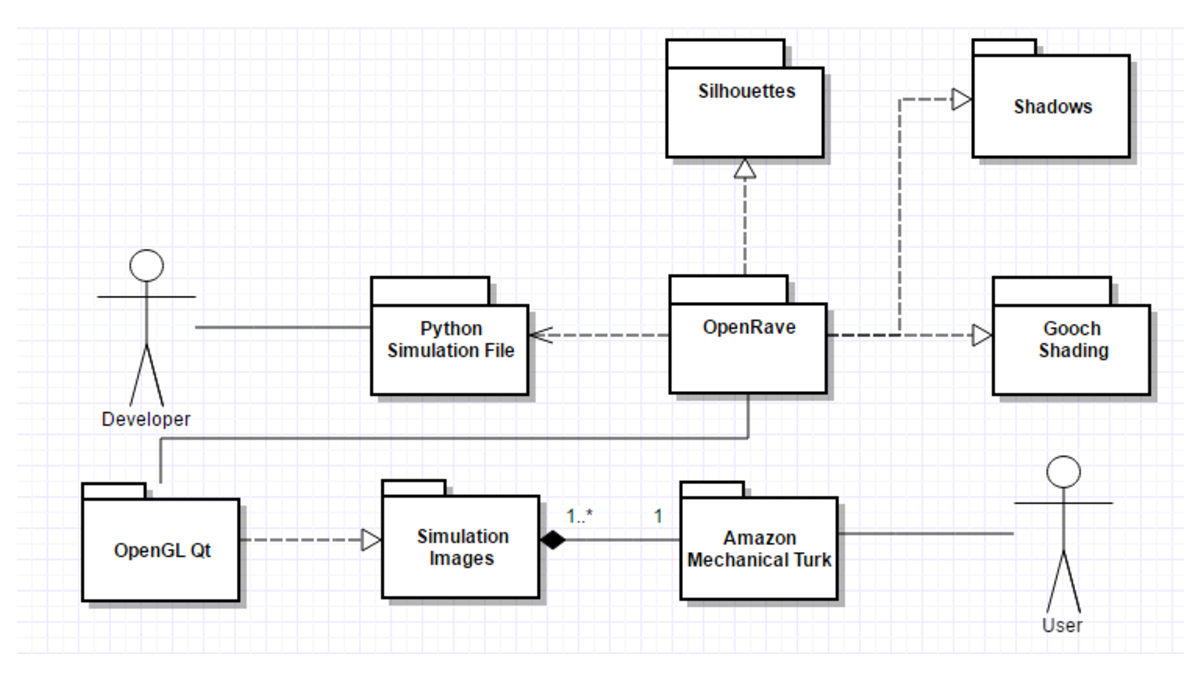
\includegraphics[scale=0.8]{designdoc_v1/Gooch_Shading_context.eps}
  \caption
{ \newline \hspace{\linewidth}
Context Viewpoint Diagram that shows relation of Gooch Shading to OpenRave}
  \label{fig:Gooch_Shading_context}
\end{figure}

\paragraph{Design View}
Gooch Shading will be implemented into OpenRave assuming that OpenRave is indeed the renderer.
A successful Gooch Shading implementation will use warm and cool coloring to help improve object geometry (which will be displayed by Qt).
Improved object geometry means improved simulation images for users of the Amazon Mechanical Turk.
The updated images will aid user confidence in how they answer the mechanical turk questions which will improve the data collected.

\subsubsection{Compositional Viewpoint}

\begin{figure} [H]
  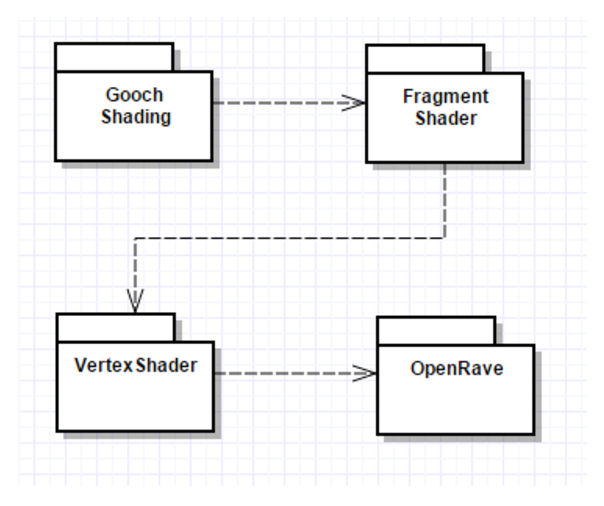
\includegraphics[scale=0.9]{designdoc_v1/Gooch_Shading2_composition.eps}
  \caption
{ \newline \hspace{\linewidth}
Compositional Viewpoint Diagram that shows the flow of Gooch Shading implementation to OpenRave}
  \label{fig:Gooch_Shading2_composition}
\end{figure}

\paragraph{Design View}
This implementation of Gooch Shading makes use of the following entities: the vertex buffer, the fragment buffer, and the renderer (OpenRave). 
OpenRave will supply relevant variables (camera position, object position, light position, colors, etc.) to the vertex shader.
The vertex shader calculates the light position and passes its variables to the fragment shader.
The fragment shader is the entity that shades the 3D objects.
In it, it calculates the diffuse lighting along with the augmented warm and cool colors that will shade the object.
The augmented warm and cool colors are determined by the object's original color and the Gooch Shading weight.
After that, linear interpolation is done on the two augmented colors to determine what the final color will be for that fragment.
In GLSL, linear interpolation can be done using the mix() function.
This shading will highlight the entire object leaving no completely "blacked out" areas.

\newpage

\subsubsection{Logical Viewpoint}

\begin{figure} [H]
  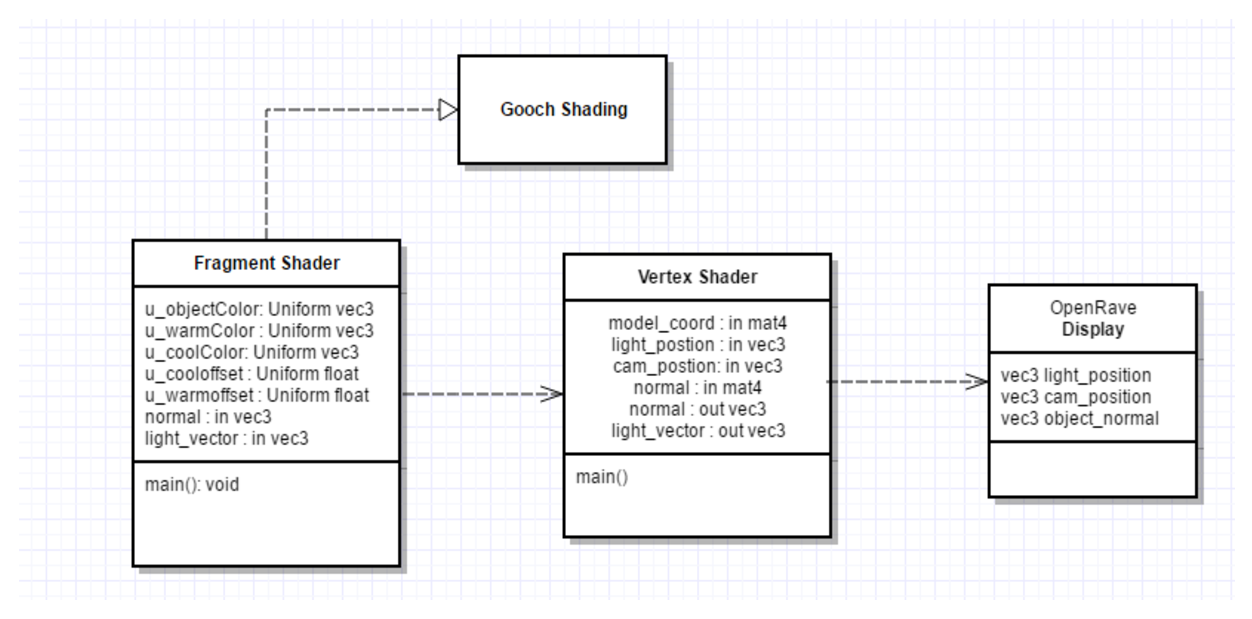
\includegraphics[scale=0.8]{designdoc_v1/Gooch_Shading_composition.eps}
  \caption
{ \newline \hspace{\linewidth}
Logical Viewpoint Diagram that shows the implementations of Gooch Shading}
  \label{fig:Gooch_Shading_composition}
\end{figure}

\paragraph{Design View}
In the code, the Gooch Shading inputs will come from the display function of the renderer.
The display function obviously holds many variables, but will only pass the following variables to the vertex shader:
\begin{itemize}
\item Camera position.
\item Object normal vector.
\item Light position.
\item Object position (model coordinates).
\item Colors (warm, cool, object original).
\end{itemize}

The warm and cool colors are determined by the developer and the object color is supplied by the python file passed into OpenRave.
The camera and object position are needed to determine the object's world coordinates (which is done in the vertex shader).
All these variables are written in GLSL.
GLSL can be used if the version of OpenGL on the system is 2.0 or above; the current version on the system will be updated to meet this requirement.
The vertex shader calculates the light vector using the object's world coordinates and the light position. 
Afterwards, it outputs the colors (warm, cool, object), the light vector, and the object's normal vector to the fragment shader.
The fragment shader will then determine the diffuse lighting for the object (diffuse lighting is the dot product of the object's normal vector with the light vector).
Following that, it augments the warm and cool colors (using the formula: color + object\_color*gooch\_shading\_weight), and then linearly interpolates between them using the GLSL mix() function \cite{glslmix}.
This interpolation determines the shade coloring for that specific fragment of the object.

\newpage

\subsection{Requirement: Silhouettes}
\large{By Matthew Huang}

\normalsize
\subsubsection{Design Concerns}
Silhouettes need to give the 3D shapes in the simulation solid borders so that the objects in the scene can be differentiated from each other.
The silhouettes need to be working in situations where objects overlap with each other and under multiple viewpoints. 
The algorithm for how the silhouettes are drawn needs to be clear.

\subsubsection{Design Stakeholders}
Cindy Grimm, Justin Bibler, Matthew Huang, and Daniel Goh

\subsubsection{Context Viewpoint}

\begin{figure} [H]
  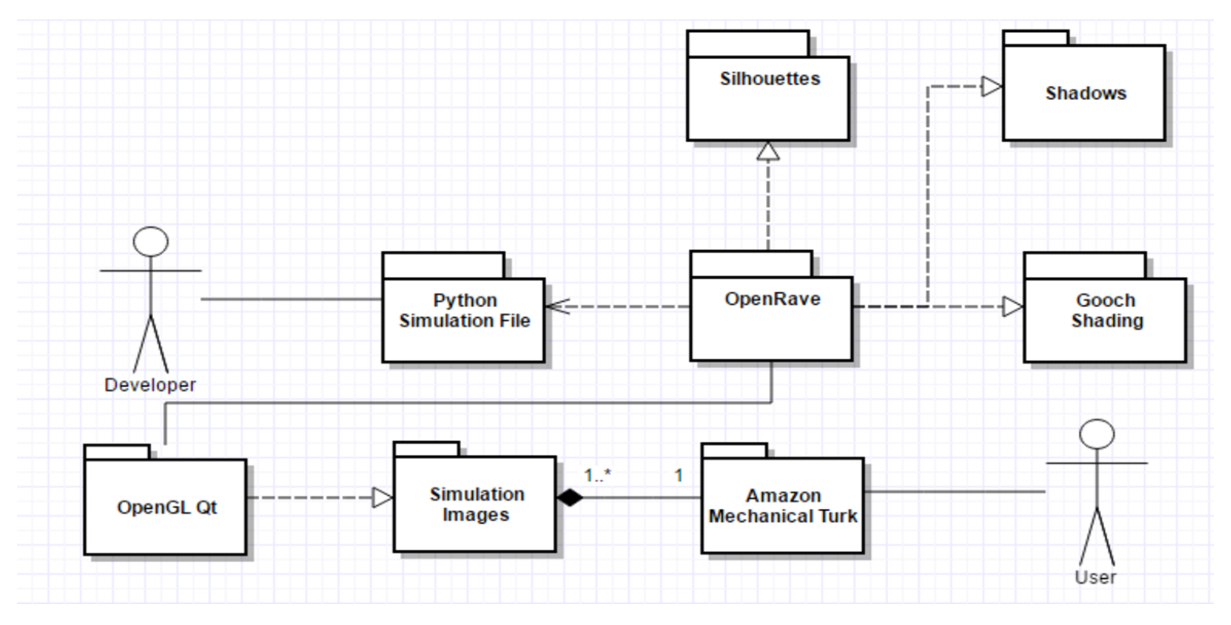
\includegraphics[scale=0.8]{designdoc_v1/Silhouettes_context.eps}
  \caption
{ \newline \hspace{\linewidth}
Context Viewpoint Diagram that that shows relation of silhouettes to OpenRave}
  \label{fig:Silhouettes_context}
\end{figure}

\paragraph{Design View}
The context viewpoint for silhouettes is essentially the same as the one for shaders.
That is to say, its end goal is to improve the end user experience by enhancing the images sent to the Amazon Mechanical Turk.
Additionally, it will also be implemented in OpenRave.
Where it differs, however, is in how it affects the simulation images.
Instead of highlighting 3D object geometry like the Gooch Shading will do, silhouettes will emphasize an object's borders (I.E. where an object begins and ends).
These silhouettes are meant to help users differentiate between objects in the simulation images.

\subsubsection{Compositional Viewpoint}

\begin{figure} [H]
  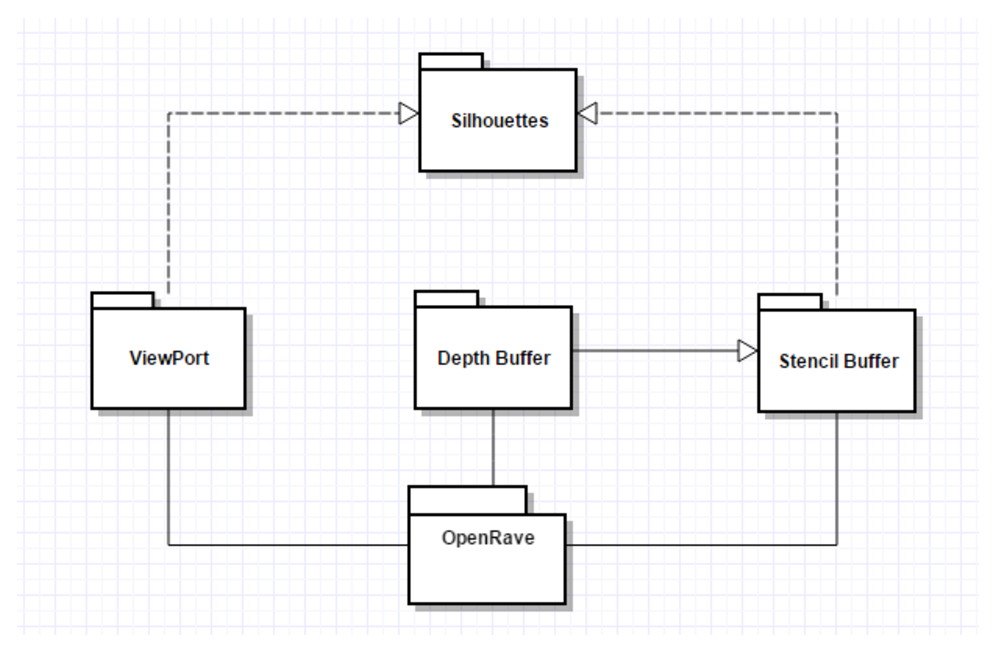
\includegraphics[scale=0.9]{designdoc_v1/Silhouettes_composition.eps}
  \caption
{ \newline \hspace{\linewidth}
Compositional Viewpoint Diagram that show relationship of Silhouettes}
  \label{fig:Silhouettes_composition}
\end{figure}

\paragraph{Design View}
Silhouettes will be implemented using a combination of the Stencil Buffer along with manipulation of the view port.
The Stencil Buffer is an optional extension of the depth buffer; both of them can be enabled in OpenRave using the glEnable() function (I.E. glEnable(GL\_STENCIL\_TEST) \cite{depthstencils}.
The Stencil Buffer gives you control over which fragments of the object should be drawn and which shouldn’t.
The viewport allows you to translate your objects in windows coordinates (I.E. pixels).
The basic algorithm to implement these silhouettes is to move the object in one direction (x, y, -x, or -y), draw the object with the stencil buffer enabled, and then repeat until you have drawn in all four directions.
The amount you move the object will affect how large of a silhouette is made.
To draw a solid color silhouette (I.E. black), draw the silhouette using a solid color version of the object.
Additionally, because the stencil buffer gives you control over what fragments of the object are drawn, overlapping objects are dealt with easily.

\newpage

\subsubsection{Algorithm Viewpoint}
Silhouette Algorithm pseudo-code implementation

\begin{lstlisting}
glEnable(stencil buffer)
glDisable(depth buffer)
glDisable(color buffer)
Clear(stencil buffer)
glStencilFunc(Always Pass)	//tell the stencil buffer to let all fragments pass
glStencilOp(Increment)		//tell stencil buffer to increment on acceptance
glViewPort(Move +y)	//Move object by some amount of pixels in the y direction
Display(object)		//render object
glViewport(Move -y)
Display(object)
glViewport(Move +x, +y)
Display(objecT)
glViewport(Move -x)
Display(object)
glViewport(Move +x)
glEnable(color buffer)
glEnable(depth buffer)
glStencilFunc(Pass if value is 2 or 3)
\end{lstlisting}

\paragraph{Design View}
The pseudo-code created above was based off of the algorithm available on the opengl silhouette edges webpage \cite{siledges}.
In general, the algorithm is easily to follow if you know how to manipulate the stencil buffer and the view port (which we do).
To summarize, glViewport() is the function that will be translating the object in windows coordinates (I.E. pixels), glStencilFunc() is the function that gives the developer control over which fragments to render, and glStencilOp gives the developer control over what happens to the stencil value of the fragment if it's accepted.
The Display() function will presumably be somewhere in OpenRave and will be the function that ultimately renders the object.
Importantly note that in total, Display() is called four times in the algorithm meaning that the object must be rendered four times to create the silhouette.
If this factor affects the runtime of the system to the point where performance benchmarks are not met, the algorithm should be changed.

\newpage

\subsection{Requirement: Creation of Online Survey}
\large{By Matthew Huang}

\normalsize
\subsubsection{Design Concerns}
The modifications made to the current OpenRave system (Gooch Shading, silhouettes, and shadows) may slow the system down.
As a requirement, the modified system must run at a minimum 30 frames per second (fps).
As a requirement, the modified system must render the initial simulation image within 30 seconds.
To assist with these requirements, the debugger shall have the ability to track function calls.

\subsubsection{Design Stakeholders}
Cindy Grimm, Justin Bibler, Matthew Huang, and Daniel Goh

\subsubsection{Context Viewpoint}

\begin{figure} [H]
  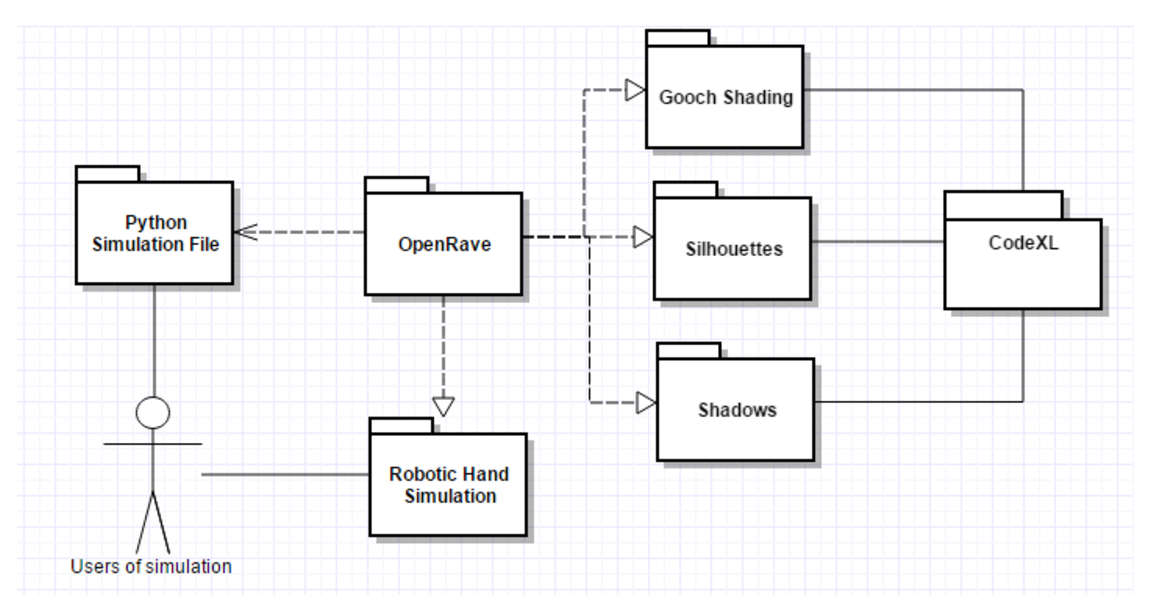
\includegraphics[scale=0.9]{designdoc_v1/CodeXL_Context.eps}
  \caption
{ \newline \hspace{\linewidth}
Context Viewpoint Diagram that shows relationship of CodeXL}
  \label{fig:CodeXL_Context}
\end{figure}

\paragraph{Design View}
CodeXL will be primarily used to track our Gooch Shading, silhouette, and shadow implementations.
Its main goal is to monitor the effect that these three implementation have on the OpenRave simulation.
If the implementations cause the robotic hand simulation to drop below 30 frames per second, CodeXL should be able to pinpoint where the cause originated from.
The goal of this is to ensure a pleasant and smooth experience for the users of the robotic hand simulation.

\subsubsection{Dependancy Viewpoint}

\begin{figure} [H]
  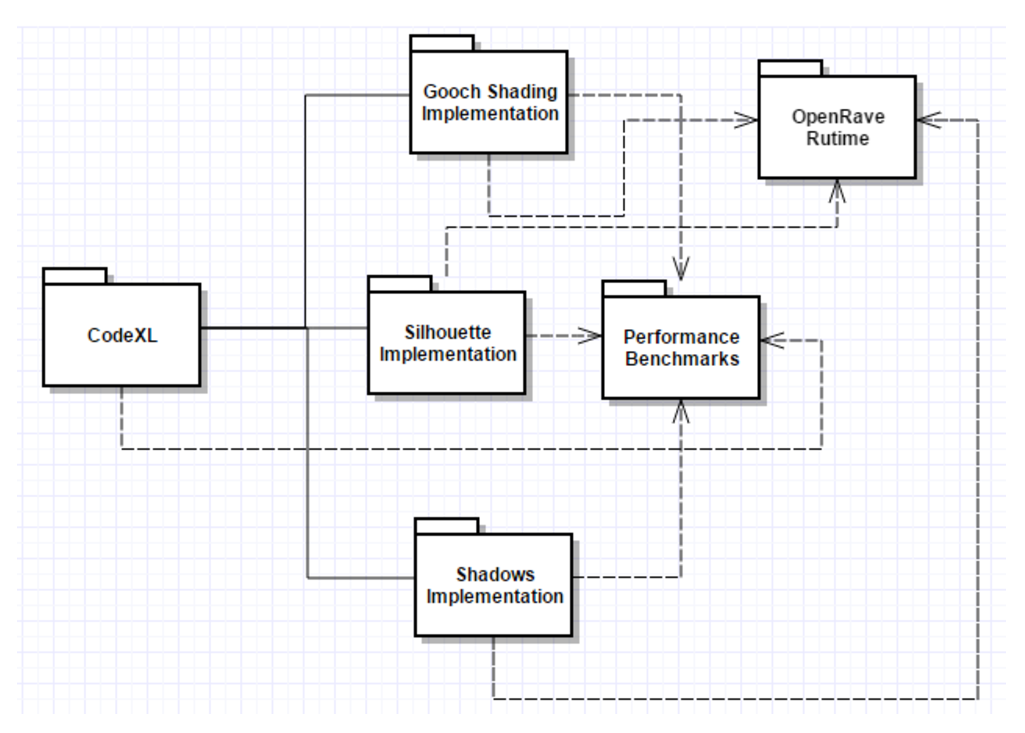
\includegraphics[scale=0.9]{designdoc_v1/CodeXL_Dependency.eps}
  \caption
{ \newline \hspace{\linewidth}
Dependancy Viewpoint Diagram that shows dependencies of CodeXL}
  \label{fig:CodeXL_Dependency}
\end{figure}

\paragraph{Design View}
How CodeXL monitors the three implementations will depend on the performance benchmarks for the whole system.
If the implementations are in and the performance benchmarks are met, inefficient function calls or other issues brought up by CodeXL may be ignored.
If the implementations bring the system down below performance benchmarks, CodeXL will have to display what is happening in the system that is causing it to slow down.
Causes like large amounts of the same function calls, long running functions, and other bugs should be tracked.
Specifically, if the frames drop below 30fps, CodeXL should be able track which implementation (or which combination of implementations) is causing the most performance loss.
If the silhouettes are causing significant performance loss, they will be the first to be refactored since there are many ways to implement silhouettes. 
Gooch Shading is less flexible in its implementation so refactoring it will have a lower priority (shadows is somewhere between silhouettes and Gooch Shading).

If OpenRave takes more than 30 seconds to render, problems likely exist in how we initialize our scene.
In this situation, CodeXL will be used to primarily track activity in the Display function since that is the function the renders the initial scene.
Other object initialization functions will not be tracked since we assume that they are pulled from libraries we have no control over.
Additionally, performance benchmarks will only be changed as a last resort (I.E. we cannot refactor our implementations anymore).

\subsubsection{Interface Viewpoint}

\begin{figure} [H]
  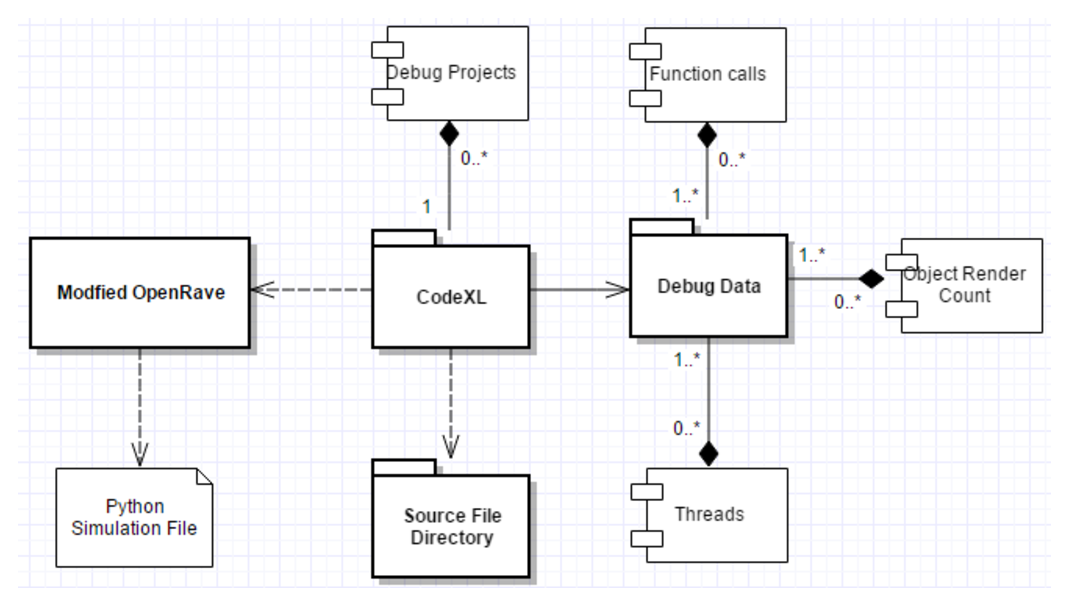
\includegraphics[scale=0.9]{designdoc_v1/CodeXL_Interface.eps}
  \caption
{ \newline \hspace{\linewidth}
Interface Viewpoint Diagram that shows the interface relations of CodeXL}
  \label{fig:CodeXL_Interface}
\end{figure}

\paragraph{Design View}
To monitor OpenRave, create a debug project in CodeXL and set the OpenRave executable as the debug project's executable.
Additionally, provide the python simulation file as a command line argument and set the source file directory to where the python file lives (this is all done in creating the debug project).
Afterwards, execute the debug project and CodeXL will display debug information such as rendered objects, created threads, and function calls (if you turn that on).
Note, however, that tracking function calls slows down CodeXL significantly so it shouldn't be used for basic testing.
Past that, CodeXL also provides access to the source code currently running directly on the CodeXL GUI.

\newpage

%Justin's section
\subsection{Requirement: Shadows}
\large{By Justin Bibler}

\normalsize
\subsubsection{Software Design Description}
Our client requires us to add shadows into the simulation's graphics.
The addition of shadows will improve the overall graphics of the simulation, which will help a user better understand where an object is within a 3D space.

\subsubsection{Design Stakeholders}
Justin Bibler, Matthew Huang, and Daniel Goh

\subsubsection{Design Concerns}
All stakeholder share similar design concerns.

Shadows design concerns:
\begin{enumerate}
\item Will our shadow implementations have a major impact on FPS.
\item Will our shadows be too pixelated.
\item Will users be able to better understand where an object is because of our shadow implementation.
\end{enumerate}

\newpage

\subsubsection{Design Views}
\paragraph{Interface Design}
This section is dedicated to talking about the graphical quality of our shadow implementation.

\subparagraph{Design Concerns}
Interface design concerns:
\begin{enumerate}
\item Will users be able to better understand where an object is because of our shadow implementations.
\item Will our shadows be too pixelated.
\end{enumerate}

\subparagraph{Design Elements}
\textbf{Name}
Shadow Interface.

\textbf{Type}
Visual, or Graphic.

\textbf{Purpose}
Shadows with the simulation exist to better help users understand an objects location within a 3D space.

\textbf{Relationship}
The quality of the visuals rely heavily on the design discussed later within the Algorithmic implementation of shadows.

\textbf{Interface attribute}
Depending on the implementation in the algorithm viewpoint, every 3D model within the simulation should have a shadow.
Whether or not the shadow is visible is dependent on if there is a surface that the shadow volume collides with.
These shadows should have minimal pixelation.
In addition, the shadows should be relatively close in shape to their original models, as to not confuse what shadow is projected out from what object.
All of this is done so that the users will easily be able to understand what shadow is related to what object, and to receive a better understanding of the 3D environment in the simulation.

\newpage

\paragraph{Algorithm Viewpoint}
The idea of the shadow volume algorithm is to extend the silhouettes of objects that are in contact with light sources into volumes.
And whenever another object falls within the shadow objects volume, it is rendered in a different way. \cite{shadow}

\subparagraph{Design Concerns}
Algorithm design concerns:
\begin{enumerate}
\item Will the algorithm be costly to the simulation's FPS.
\end{enumerate}

\subparagraph{Design Elements}
\textbf{Name}
Algorithmic implementation of shadows.

\textbf{Type}
Algorithm, or method.

\textbf{Relationship}
Shaders, and the Shadow Interface.

\textbf{Design Constraints}
The implementation of shadows will most likely rely on the knowledge we gain from implementing warm cool shaders into the simulation.
That knowledge will allow us to better understand how the simulation is being rendered, making it easier for us to adjust and change certain shaders.
Another constraint that we have is that there is a relatively small amount of documentation related to OpenRave and OpenInventor.
This makes it difficult to find exactly where we need to implement shaders to get our desired results.

\textbf{Processing Attribute}
The bases of the algorithm will be using the depth fail test.
This will be done by first rendering all the objects in the scene into the depth buffer.
From here, we create shadow volumes for each object based on the objects silhouette projected into infinity relative to where the light is striking the object.
Then we render the volume into the stencil buffer based off the depth fail test.

Depth fail test:
\begin{enumerate}
\item If the depth test fails while rendering back facing polygons of the shadow volume, we increment the stencil buffer.
\item If the depth test fails while rendering the front facing polygons of the shadow volume, we decrement the stencil buffer.
\item Nothing happens if the test passes, or the stencil test fails.
\end{enumerate}

This depth fail test is conducted for each shadow volume.
Once the tests have concluded, the scene will be rendered into the viewport.
However, only the objects, or parts of objects, that have a stencil buffer value of zero will be rendered without alterations. \cite{shadow}

\newpage

\subsection{Requirement: Measuring the Simulation's FPS}
\large{By Justin Bibler}

\normalsize
\subsubsection{Software Design Description}
Our project requires us to measure and analyze the runtime and FPS of our altered simulation.
This is done so that we can ensure that our additions fulfill our performance metrics: the simulation must maintain an average 30 FPS.
 If we are unable to reach this metric our implementations will be considered incorrect, and will require revisions.

\subsubsection{Design Stakeholders}
Justin Bibler, Matthew Huang, and Daniel Goh

\subsubsection{Design Concerns}
All stakeholders share similar design concerns.

Requirement design concerns:
\begin{enumerate}
\item Failing to meet our target FPS and runtime will result in revisions of our implementations.
\item Will our measurements be accurate for the majority of computers.
\item Software used for measuring may cost money.
\end{enumerate}

\newpage

\subsubsection{Design Views}
\paragraph{Information Viewpoint}
The purpose of this viewpoint is describe how information will be gathered, and how it will be analyzed.
Our team will be using an external tool to obtain data related to the simulation's FPS.
 FRAPS will be used to examine the FPS and export the information into a file to be analyzed.

\subparagraph{Design Concern}
Interface viewpoint concerns:
\begin{enumerate}
\item FRAPS is paid software.
\item Will our measurements be accurate for the majority of computers.
\end{enumerate}

\subparagraph{Design Elements}
\subparagraph{Name}
Method of analyzing and collecting FPS data.

\textbf{Type}
Method.

\textbf{Purpose}
Data collected will be analyzed to ensure that our implementations into the simulation meet our requirements.

\textbf{Data attribute}
FRAPS will be used to capture data related to FPS, this will be done by using the benchmarking tools that come with the software.
We will run this test for one minute ten times, on five different sample simulations with our updated graphics.
This data will be exported into a file, from here we will analyze the data by finding the mean and median across all executions.
If these values are within a certain standard deviation of 30 FPS, our implementation will be considered correct.

\textbf{Author}
FRAPS is owned by Beepa.\cite{fraps}

\subsubsection{Rational}
Even though FRAPS is a paid software I've decided that it be best if we use it.
It's ability to export data into a file allows our group to easily obtain and analyze data.
Furthermore, our concern related to the validity of the data stems from the fact that our group members own above average computers.
Thus, testing on our computers would most likely be inaccurate relative to the average computer.
To circumvent this problem we plan to do most of our testing on the computers on the OSU campus.

\newpage

\subsection{Requirement: Code Maintainability}
\large{By Justin Bibler}

\normalsize
\subsubsection{Software Design Description}
The goal behind code maintainability is to increase the cost effectiveness of changes being made to a system. \cite{maintain}
Our group has made this a requirement because our client wishes to be able to easily change, or add into our implementations.
The primary logic behind this design is the use of good programming practices such as documentation, and commenting, but also the use of external resources which are described within the viewpoint below.

\subsubsection{Design Stakeholders}
Justin Bibler, Matthew Huang, and Daniel Goh

\subsubsection{Design Concerns}
All stakeholders share similar design concerns.

Requirement design concerns:
\begin{enumerate}
\item Cost of static code debugging tools.
\item Lack of documentation for preexisting code.
\item Lack of comments for preexisting code.
\end{enumerate}

\newpage

\subsubsection{Design Views}
\paragraph{Resource Viewpoint}
External resources will be used to help us maintain and upkeep our code quality.
The first resource we will be using, which within today's standard is almost a necessity, will be GitHub.
GitHub is a repository that is used for code version control.
Secondly, we will be using Cppcheck.
Cppcheck is a static code analysis tool that examines code for bugs that a compiler may not catch.

\subparagraph{Design Concern}
Interface viewpoint concerns:
\begin{enumerate}
\item Using Cppcheck may bring about problems within preexisting code not written by us.
\end{enumerate}

\subparagraph{Design Elements}
\textbf{Entities}
Both GitHub, and Cppcheck are free to use by the public

\textbf{Name}
Resources for Code Maintainability.

\textbf{Type}
External resource.

\textbf{Function}
GitHub will be used for version control of the code.
Cppcheck will be used to assist in finding and fixing bugs within our code implementations.

\textbf{Resource attribute}
GitHub is important because it will allow us to have easy access to past versions of code.
Using GitHub is like a safety net that will allow us to be free with how we edit the code, because in the case that we create a massive new problem;
it is very easy for us to pull an earlier version of the code to work on.
Along with this GitHub also has a built in wiki that will be used to record and document our new implementations and functions within the code.
Allowing for easy reference for ourselves and our client.\par
Cppcheck will be used to examine our new implementations into the code.
Using this tool will allow us to quickly find and eliminate bugs within the code.
Few amount of bugs within code will allow us to make changing and creating new implementations safer and easier.

\textbf{Author}
GitHub is owned by GitHub, Inc.
Cppcheck is open source.

\subsubsection{Rational}
The reason Cppcheck was decided upon was because it is open source and free, other static analysis tools cost a significant amount of money.
Which makes the Cppcheck option the best for our group.
Also, the design behind "Code Maintainability" can be improved by the use of the resources I talked about. 
However, a large part of it will rely more on how well our group documents the improvements we make through resources such as GitHub.
It'll be important while we go forward to document both how we implemented our improvements, and how to use our improvements.
This is because, as mentioned in the Requirement concerns, we are working off preexisting code.
Thus, our client will need some sort of good reference of how to navigate the code, and how to make proper adjustments.


\newpage
% Daniel's Section
\subsection{Requirement: Creation of Online Survey}
\large{By Daniel Goh}

\normalsize
\subsubsection{Software Design Description}
This requirement is established to allow participants to provide their input to determine if the team's visual enhancement to the robotic simulation has improved from its initial state.
This will be fulfilled by running online surveys.
Google Forms is the selected platform to run the online survey.

\subsubsection{Design Stakeholders}
Justin Bibler, Matthew Huang, and Daniel Goh

\subsubsection{Design Views}
\paragraph{Interface Viewpoint}
\subparagraph{Design Concern}
Google Forms is the selected service that will be utilized to carry out the online survey. 
The design concern for the online survey will include if participants will be able to understand the questions of the online survey and select their choice of better visuals. 
\vspace{3mm}

\subparagraph{Design Elements}
\textbf{Name}
Survey Interface Understandability

\textbf{Type}
System used to assess resulting visuals for the robot grasping simulation. 

\textbf{Purpose}
This element exists to help guide the creation of an online survey that is easily understood and usable by the participants. 

\textbf{Function}
Google Forms \cite{googleforms} is a matured survey platform that allows unlimited number of questions and the function to attach images to the created survey.
Participants will be able to select a picture or answer based on the questions presented. 
The questions will cover the aesthetic aspects between pictures, the presence of shadows between pictures, and identification of object relativity or position within the picture. 

\textbf{Interface}
Methods of interaction provided by Google Forms include:
\begin{itemize}
\item Allowing participants to view attached images for a question
\item Allowing participants to select a single answer or image for a question
\item Allowing participants to select multiple answers or images for a question  (checkboxes)
\item Participants responses will be stored as a data file within Google Forms and exportable to Google Sheets(.csv files, comma separated value files)
\end{itemize}

Users should not be overwhelmed by information in the interface while taking the survey.
Survey questions should ask the user for a specific opinion (e.g. questions asking about presence of shadows should only focus on asking about shadows and nothing more) at a time and ideally have no more than one sentence \cite{SMquestions}. 
Survey questions should be designed to be balanced and not biased.
For example, stating the left visual is the improved visual in the question while asking the user to select the better visual is a form of bias.  

\newpage

\subsection{Requirement: Analysis and Visualization of Collected Data}
\large{By Daniel Goh}

\normalsize
\subsubsection{Software Design Description}
The data collected from the online survey will require analysis to determine if the team's visual enhancement to the robotic simulation has improved from its initial state.
The data will need to be organized and analyzable by the stakeholders.
Google Sheets will be used to analyze and visualize the collected data.

\subsubsection{Design Stakeholders}
Justin Bibler, Matthew Huang, and Daniel Goh

\subsubsection{Design Views}
\paragraph{Information Viewpoint}
\subparagraph{Design Concerns}
Google Sheets \cite{googlesheets} is the selected platform to parse and visualize the data collected from the online survey. 
The design concern includes if the data collected can be analyzed and visualized meaningfully to reflect the collective participants’ responses.
\vspace{3mm}

\subparagraph{Design Elements}
\textbf{Name}
Data Visualization

\textbf{Type}
System for data parsing and visualization that supports Google Forms 

\textbf{Purpose}
The element exists to help guide the use of Google Sheets to create data visualizations.

\textbf{Data Attribute}
As Google Forms and Google Sheets are under one ecosystem, Google Sheets have access to parse the data collected directly into Google Forms. 
The resulting data content will contain individual responses on a single spreadsheet. 

Questions asked will be represented on the first horizontal row. 
Participant's responses are time stamped and is represented as a row for each individual. 
The participant's responses (answer to each questions) are recorded below the questions. 

\begin{center}
\begin{table}[H]
\caption{Spreadsheet example with data}
\begin{tabular}{ | m{5em} | m{15em} | m{7em} | m{7em} | m{7em} |  m{7em} | } 
\hline
\textbf{Respondent}  & \textbf{Time stamp}  & \textbf{Question 1} & \textbf{Question 2} & \textbf{...} & \textbf{Question N} \\ \hline
1 & 11/12/2016 20:28:39 & Choice 1 & Choice 2 & ... & Choice 2 \\ \hline
2 & 11/13/2016 1:55:37 & Choice 1 & Choice 2 & ... & Choice 1 \\ \hline
3 & 11/13/2016 11:56:02 & Choice 2 & Choice 2 & ... & Choice 2 \\ \hline 
4 & 11/15/2016 23:52:12 & Choice 1 & Choice 2 & ... & Choice 1 \\ \hline 
5 & 11/18/2016 15:51:32 & Choice 1 & Choice 1 & ... & Choice 2 \\ \hline 
\end{tabular}
\newline
\label{table:Example}
\end{table}
\end{center}

The selected data analysis method that will be used to determine the project's success will be based on frequency among all respondents \cite{SManalysis}. 
An example model that represents the frequency method is as follow:

\begin{equation}
\frac{Number Of Choice 1 Occurrence For Question 1}{Total Respondents} = x\%
\end{equation}

\vspace{3mm}
In this example, Choice 1 for Question 1 is the visuals with enhanced shadows implementation. 
x will need to be more than 79 in order for shadow implementations to be considered a success.

The data collected will be converted into visualizations using the charting functions provided in Google Sheets. 
For ease of understandability and quick visualization, the pie chart charting option will be used to display the collective responses. 

\newpage

\subsection{Conclusion}
In conclusion, this design document will be used as a plan of action as we go forward with our implementation.
This document is not set in stone; it may change as needed as we begin making changes to the code.
However, it is important to note that our requirements will not change; only our approach to tackle the requirements may change.

\vfill

\noindent\begin{tabular}{ll}
\makebox[2.5in]{\hrulefill} & \makebox[2.5in]{\hrulefill}\\
Cindy Grimm & Date\\[4ex]% adds space between the signatures
\makebox[2.5in]{\hrulefill} & \makebox[2.5in]{\hrulefill}\\
Justin Bibler & Date\\[4ex]% adds space between the signatures
\makebox[2.5in]{\hrulefill} & \makebox[2.5in]{\hrulefill}\\
Matthew Huang & Date\\[4ex]% adds space between the signatures
\makebox[2.5in]{\hrulefill} & \makebox[2.5in]{\hrulefill}\\
Daniel Goh & Date\\
\end{tabular}

\end{flushleft}

\section{Design Document Update}

\begin{center}
\begin{table}[H]
\caption{Table showing the design that is changed (Design), and what happened to it (Change Details).}
\begin{tabular}{ | p{0.2\linewidth} | p{0.7\linewidth} | }
\hline
\textbf{Design}  & \textbf{Change Details} \\ \hline
Warm Cool Shading & 
Warm Cool shading is still done in vertex and fragment shaders, but those shaders are now created by SoShadowGroup.cpp. 
Therefore, the Warm Cool shading code is now in the SoShadowGroup library. 
Additionally, the Warm Cool shaders now adapt to the object's original color. 
This was necessary to prevent bad color mixtures such as blue and orange. 
Further details on how this was done can be found in the design document. \\ \hline
Silhouettes & Silhouettes are now done using the silhouette lines method. 
In other words, the silhouettes are rendered using GL\_LINES instead of polygons. 
This was done to keep consistent silhouette widths throughout all the rendered objects. \\ \hline
CodeXL & Removed since the fps requirement was removed. 
Additionally, CodeXL only works on Windows (our system runs on Ubuntu 16.04) and testing was done better by simply running the system on different machines. \\ \hline
Online Survey Creation & 
The online survey creation is changed to use Qualtrics instead of Google Forms.
Most of the design remain the same, except for some additions that come with Qualtrics' survey features.
The design of the online survey utilized blocks to separate questions across pages. \\ \hline
Data Analysis and Visualization & 
The data analysis and visualization tool is changed to use Qualtrics instead of Google Sheets.
The design of data analysis and visualization remains the same. \\ \hline
Shadows &
The design was changed to use the built in SoShadowGroup class, which creates variance shadow maps.
This design change decisions was made because creating our own shadows would turn out to be very difficult.
When there was already a class in coin3d that generated shadows.
Thus, it was of our best interest to use resources already available to us instead of wasting time creating our own. \\ \hline
Measuring FPS &
Matthew and Justin overlapped their design of the FPS requirement.
However, the requirement was removed so no testing of the FPS was ever done.
Along with the this design becoming unnecessary the software that was planned to be used was Windows only. \\ \hline
Code Maintainability &
We maintained good version control of our code changes throughout the project.
However, cppcheck was never used on the code.
The usage of cppcheck would prove to be meaningless.
We were simply adding to existing code, and not making our own completely unique code.
Thus if we would have used cppcheck we would be refactoring a significant amount of code not written by us, and code that we may not fully understand.
Thus, it would be dangerous as we might be unable to properly document these changes. \\ \hline
\end{tabular}
\newline
\label{table:DesignDocumentUpdate}
\end{table}
\end{center}

\newpage

\section{Tech Review}

Refer to next page for the initial technology review document.

\newpage

\onecolumn

\begin{titlepage}
\null
\vspace{20mm}

\begin{flushleft}
\begin{bfseries}
	\vskip2mm
	\Huge{Technology Review for\\ Better Graphics For A Robotics Grasping GUI}\\
	\vspace{30mm}
	\textbf{\huge Shady Robots} \\
	\vskip2mm
	\large{Group 12}
	\vskip5mm
	\Large{Justin Bibler \\
	Matthew Huang \\
	Daniel Goh \\}
\end{bfseries}

\vspace{15mm}
\Large{CS461: Senior Software Engineering Project} \\
\Large{Fall 2016} \\

\vspace{10mm}

\today

\vfill

\begin{normalsize}
{\bf Abstract:}
Our client is using a simulation to create visuals that are used for online data collection.
This simulation is using outdated libraries which result in outdated graphics.
We, as the supplier, compare and contrast the different technology and methods that will be used during the phase of the project to ensure the project's success.
\end{normalsize}
\end{flushleft}
\end{titlepage}

\subsection{Introduction}
\vspace{3mm}
The technology review document is used to determine the best approach of implementation for the project. 
Clause 2 lists the references made to other documents.
Clause 3 lists each team member's role in the project and accomplishment goals.
Clauses 4 to 6 are the technology review that is carried out by each team member.
Clause 4 reviews the technology to be used to carry out runtime analysis. performance benchmarks, and best practices to implement shadows.
Clause 5 reviews the best practices to implement shaders, best practices to implement silhouettes, and technology to be used to ensure maintainability of the project's source code.
Clause 6 review usability inspection methods, run user interviews, and tools to analyze the respondents data.

\newpage

\subsection{Roles}

\subsubsection{Justin Bibler}
My roles within this project vary from each other, and are not one cohesive singular responsibility.
I have two responsibilities that have a conclusive end, and a responsibility that is maintained throughout the entire project.
The first of the two conclusive responsibilities that I have is to locate where in the code the rendering is happening.
This responsibility is critically important to the entirety of the group, as without knowledge of the location of the rendering function it is difficult to implement shaders.
Secondly, I will be overseeing the implementation of the shadows.
Shadows help define where 3d objects are within a computer simulation, thus our client requested them to be implemented to improve the current graphics.
Finally, my last responsibility is to assure code maintainability.
This means that once our group has finished with the project our additions to the code will be well documented, commented, and easily understandable.
Making it easy for our shader implementations to be changed and adjusted easily to fit our client's needs. \par
Within the "Identification of Rendering loop, Methods of code maintainability, and Shadows" section I compare and contrast three different methods and tools available to conduct and maintain my responsibilities.
How the comparison of methods and tools will be conducted is: I will first explain what the responsibility is and it's relevance to the group and the project.
I will then list a tool or method and how it is used or conducted.
Next, I will list and analyze the benefits and negatives of a tools usage.
At the end of each section I discuss my opinion on the usage of the method.
Finally, after listing all of the available different method and tools I will give my verdict on what will be used.

\subsubsection{Matthew Huang}
In this team, I'm responsible for the non photorealistic shaders, the silhouettes, and the runtime performance of the modified simulation.
For the shaders, I must make sure that they improve the geometric shape of each object in the simulation.
For the silhouettes, I must make sure that they clearly show where an object's borders are so that user can differentiate shapes from each other.
For the runtime performance, I must make sure that our implementation does not negatively affect the frames per second that the current simulation is running at.
To ensure this, I have researched various debuggers that will help us see what our program is doing during runtime.


\subsubsection{Daniel Goh}
My role within Shady Robots is to measure the improvement that is implemented into the simulation.
I will also be running the selected inspection method to determine if the project has reached the end goal.
After running the usability inspection, I will be compiling, visualizing and analyze the data set.

Usability inspection methods will be a standard of metrics to determine if the project has reached the end goal.
The goal within this document is to compare and contrast the different available usability inspection methods, data collection tools, and analytical and visualization tools.
After reviewing the various tools, a final verdict of the review is presented at the end of each section.

\newpage

\subsection{Identification of Rendering loop, Methods of code maintainability, and Shadows}
\large{By Justin Bibler}

\normalsize
\subsubsection{Identification of Rendering loop}
Our project requires our group to make new implementations into the existing OpenRave code.
However, the location of the rendering functions within OpenRave are not entirely know to our client.
Therefore, the responsibility of locating these functions has been given to our group.
This responsibility is very important to the entirety of the project.
Most of our new implementations into the code will be reliant on the use of shaders;
 if the location of the rendering functions are unknown to us it would be extremely difficult for us to make good shader implementations.
Thus, to identify the location of the rendering functions the three most fitting methods would be: Reading Static Code, debugging, external references, and documentation.

\paragraph{Reading Static Code}
This is a very basic method in which a programmer simply reads over and reviews static code.
In this case the OpenRave source code would be read over to identify how the rendering function is working.

Benefits of Reading Static Code:
\begin{itemize}
\item The entire system can be understood at a very low level.
\item Locations of specific functions within the code can be identified.
\item Exact implementation of functions can be understood.
\end{itemize}

Negatives of Reading Static Code:
\begin{itemize}
\item This method can become very time consuming depending on the size and complexity of the code.
\item Code may difficult to read depending on how it is implemented.
\item Inefficient, a programmer will most likely have to flip around multiple source files to figure out how things are working together.
\end{itemize}

\subparagraph{Discussion}
%\vspace{3mm}
Reading static code might be too simple of a method to conduct by itself.
It would definitely help me get a good understanding of how the code is function.
However, as mentioned in the negatives of this method it may be too time consuming.
The source code for OpenRave is quite large, and I have minimal experience working on a project this large scale so it would be difficult for me to jump right in and simply read code.
Perhaps if this method were to be paired with another it could be useful.

\paragraph{Debugging}
Debugging is a process where a programmer will use tools, and programming methods to locate errors in code.
Many different forms and tools exist to conduct debugging.\cite{debugging}
Thus, I will narrow the scope down to one specific form a debugging: breakpoints, and step through.
Breakpoints stop an executable and breaks into the debugger.
This allows a programmer to analyze the code and execute debugger commands.\cite{debugging}

Benefits of Debugging:
\begin{itemize}
\item Lots of available tools.
\item Lots of available methods.
\item Powerful control over code.
\item Executable within most modern IDEs.
\end{itemize}

Negatives of Debugging
\begin{itemize}
\item Difficult to conduct on large projects.
\item Stepping through code can become time consuming.
\end{itemize}

\subparagraph{Discussion}
%\vspace{3mm}
Debugging is a good method that would help me accomplish my goal.
If I were to use a method such as breakpoints and step through code at certain points, it could become a very helpful resource to use.
However, due to the size of the program I am not exactly sure how easy it will be to debug.

\paragraph{External References, and Documentation}
Much like reading static code this is a very simple and obvious method that can be used to locate the rendering function.
This method is where a programmer will read through the available documentation to understand how the system works.
In this method a programmer will also contact other programmers who are working on the code currently, or have worked on the code in the past.
With the intention of receiving guidance on how the system works.

Benefits of External References, and Documentation:
\begin{itemize}
\item Easy to get answers to specific questions.
\item Documentation gives a good understanding of the entirety of a system.
\end{itemize}

Negatives of External References, and Documentation:
\begin{itemize}
\item There may be no documentation.
\item External sources may not exist.
\item Past programmers may be unresponsive.
\end{itemize}

\subparagraph{Discussion}
%\vspace{3mm}
It's quite obvious that this is one of the best methods.
Because I am attempting to find a specific function within the code, referring to the documentation and external sources is a good choice.
Along with this, the GitHub that is being used for OpenRave has a couple of active users so it would be relatively easy to contact another programmer who is more knowledgeable to assist me.

\paragraph{Verdict}
My verdict on methods for identifying the rendering function is that all of the proposed methods are useful.
I will most likely begin my search in the documentation then use the knowledge I gained from the documents to traverse through the source code.
This is because as helpful as the documentation will be, it's required of me to read the actual code so I will have an even better understanding of it.
If I am unable to locate the rendering function through documentation and by reading the code.
I will reach out to other programmers within the GitHub group for assistance.
As a last result, I will be using debugging techniques to traverse through the code in attempts to locate the function.

\newpage
\subsubsection{Methods of code maintainability}
The goal of creating maintainable code is to increase cost effectiveness.
This means that whenever a new change needs to be made to the system, due to how the code is a designed and constructed this change will take a minimal amount of time.\cite{maintainability}
Maintainability is important to our code, because our client wishes to have the ability to easily change and adjust our implementation of shaders into the system.
Thus our implementations into the code should use methods that allow for an increase in the ability to quickly understand and modify code.
These proposed methods are: Version Control, Refactoring, Documentation, and Commenting.

\paragraph{Version Control}
Version control has become increasingly easy to maintain with the popularity of version control tools such as GitHub.
Using version control allows for users to make copies of repositories to either use for personnel use or make altercations.
This practices gives protection to the code, such as if programmer losses or makes a devastating alteration to the code.
That programmer doesn't have to worry much, because they know they can pull unmodified working code from the repository.\cite{version}

Benefits of using Version Control:
\begin{itemize}
\item Source code is easily accessible.
\item General tests can be defined to update stable versions of code in a repository.
\item Code is safe to accidental deletion, or introductions of major bugs.
\end{itemize}

Negatives of using Version Control:
\begin{itemize}
\item There aren't really any negatives
\end{itemize}

\subparagraph{Discussion}
\vspace{3mm}
Using version control is a obvious powerful tool.
It essentially protects code from being lost or broken.
If a programmer accidentally introduces a large bug into the system, then with version control it is very easy to step back and pull older versions of the code.
In the case that a programmer accidentally deletes their code, it's easy for them to go back and simply pull it from the repository again.
Using version control most assuredly would help increase code maintainability.

\paragraph{Refactoring}
Refactoring is a process in which code is altered in a manner such that it does not change how the external behavior of the system works.\cite{refactoring}
In the case of this project, refactoring would be used after our group has created a working implementation of our clients request.
We would go back into our code, and adjust our code so that it might be smaller, more readable, and in most cases reusable.
Such as refactoring repeated code into a singular function that can be used in multiple locations of the code.

Benefits of using Refactoring:
\begin{itemize}
\item Easy to do.
\item Cuts down code size.
\item Reusable functions can be implemented and used in different locations of code.
\item Maximizes runtime.
\end{itemize}

Negatives of using Refactoring:
\begin{itemize}
\item After a lot of refactoring code can become less readable.
\end{itemize}

\subparagraph{Discussion}
%\vspace{3mm}
Refactoring is a good method to maximize code, especially when refactoring repeated code into new functions.
If I were to refactor our implementations into the code with the client's desires in mind.
I could most likely make it simple for them to adjust, and reuse functions throughout the program if they desire to change it.

\paragraph{Documentation, and Commenting}
Documentation and Commenting allows new programmers to quickly get a grasp on the code.
In the case of comments, a programmer is able to quickly understand intentions behind functions and certain operations within the code to get a better understanding of how the system works.
And documentation of the code allows a programmer to have references to many questions related to the code.

Benefits of Documentation, and Commenting:
\begin{itemize}
\item New programmers have references to the what, where, and why of code.
\item Good commenting allows a programmer to get a better understanding of the code while directly reading the code.
\item Programmers have references of how to use functions, either in the comments of a function or in the documentation.
\end{itemize}

Negatives of Documentation, and Commenting:
\begin{itemize}
\item Too much, and useless comments can make code look clustered and sloppy.
\item Writing documents can become time consuming depending on the size of system.
\end{itemize}

\subparagraph{Discussion}
%\vspace{3mm}
Early in the document I talked about how I would be using documentation to help find the rendering functions within the OpenRave code.
Thus, I personally find using documentation very helpful.
I personally would prefer to focus more heavily on documenting our additions outside of the code rather then simply using comments.
This is because documents are simply and easier reference.

\paragraph{Verdict}
Each of these methods has it's usefulness that I will utilize to keep the system maintainable.
Version control allows our group to make alterations to the code without fear of losing stable versions.
This also allows for our client to come in and make their own alterations later in the future after the project is finished.
In regards to documentation, and commenting.
I will be recording all the changes and additions we make to the source code.
This allows our group, and our client to have easy references to usable functions within the system.
Finally, I will be using refactoring when I see it fit to be used.
Our group is not expecting to make such massive alterations into the existing code that refactoring would have a major impact.
I also do not intend to refactor the currently written OpenRave code.

\newpage
\subsubsection{Shadows}
Shadows are used to help understand where in an object is within a 3d simulation.
However, the current graphics used in OpenRave do not contain shadows.
So our client has requested that we implement shadows into the current system.
My proposed methods are: Light mapping, Shadow volumes, and Shadow mapping.

\paragraph{Light mapping}
A light map is simply a texture that contains information about the lighting. 
In most cases a light map is rendered before the program is executed to speed up the programs runtime.
Essentially, this light map is blended with textures that are intended to be lit to give off an illusion of lighting, and shadows.\cite{lightmapping}

Benefits of using Light mapping:
\begin{itemize}
\item Easy to implement.
\item Can be pre-rendered to increase runtime
\end{itemize}

Negatives of using Light mapping:
\begin{itemize}
\item Lighting is not dynamic.
\end{itemize}

\subparagraph{Discussion}
Light mapping seems like a good choice for doing lighting and shading for static objects in OpenRave.
However, because the simulation contains moving 3d objects it will most likely need more dynamic shadows.

\paragraph{Shadow Volumes}
This form of shadowing takes advantage of the stencil buffer in OpenGL.
Essentially, a shadow volume is a volume in space that contains every point in which an object could be shaded.
Objects that collide with the shadow volume should generate shadowing on their surface according to the shadow volume.
This is done by rendering objects shadowed pixels with different stencil values compared to their non-shadow pixels. \cite{volume}

Benefits of Shadow Volumes:
\begin{itemize}
\item Dynamic.
\item Relatively lightweight.
\end{itemize}

Negatives of Shadow Volumes:
\begin{itemize}
\item Doesn't generate the best looking shadows.
\end{itemize}

\subparagraph{Discussion}
\vspace{3mm}
This for of creating shadows seems relatively simple for my skill level.
Along with this it's dynamic, and lightweight which are both good qualities our group is looking for in our shadow implementations.

\paragraph{Shadow maps}
Shadow mapping is kind of like light mapping.
Shadow mapping works by rendering a scene twice.
In the first render, only the depth of each fragment is computed.
In the second render, the scene is rendered normally.
However, the information computed in the first render is used to calculate whether or not an object has fragments in front of it relative to the light source.
If a fragment has a fragment from the first render blocking it, a shadow should be placed displayed. \cite{shadowMapping}

Benefits of Shadow Mapping:
\begin{itemize}
\item Shadows are dynamic.
\item Shadows will look good because they are fragment based.
\end{itemize}

Negatives of Shadow Mapping:
\begin{itemize}
\item Requires scene to be rendered multiple times.
\item Worse runtime.
\end{itemize}

\subparagraph{Discussion}
\vspace{3mm}
Shadow mapping seems great, it also seems like it would create the best looking shadows for the simulation.
However, shadow mapping would most likely greatly increase the runtime of the program and be detrimental to the FPS.

\paragraph{Verdict}
I think that the shadow volume implementation would be the best to implement into the system.
This is because it offer acceptable looking dynamic shadows, without sacrificing too much runtime and FPS.
It would be great if we could implement the shadow mapping, but the computers that the simulation will be frequently ran on does not have the best GPU.
Making shadow mapping a bad choice.

\newpage

\subsection{Non photorealistic shading, silhouettes, and optimization - run time analysis}
\large{By Matthew Huang}
\normalsize
\subsubsection{Non photorealistic shading}

\paragraph{Gooch Shading (Cool to Warm Shading)}
Gooch shading, developed by Amy Gooch, Bruce Gooch, Peter Shirley, and Elaine Cohen, is a non photorealistic shading model for rendering objects in a technical illustration style. \cite{gooch}
In Gooch Shading, the following characteristics are prominent:
\begin{itemize}
\item Edge lines are drawn with black curves.
\item 3D objects are shaded using color intensities that are far from black or white. Instead, the warmth or coolness of a color indicates its relationship to the surface normal.
\item A single light source provides white light for the object.
\item Shadowing is not shown.
\item Metal objects are shaded as if very anisotropic
\end{itemize}
The colors used in Gooch shading have distinct tones and temperatures.
The color tones are created by adding either gray to the color or by adding the color's complement to the color. The temperature of the color is defined to be warm (red, orange, yellow), cool (blue, violet, green), or temperate (red-violet, yellow-green). Shading with these colors will allow for tone scaled object color along with a warm-to-cool undertone. An example of a Gooch Shaded Object is provided in Figure 1 below. \cite{gooch2}

\begin{figure} [H]
  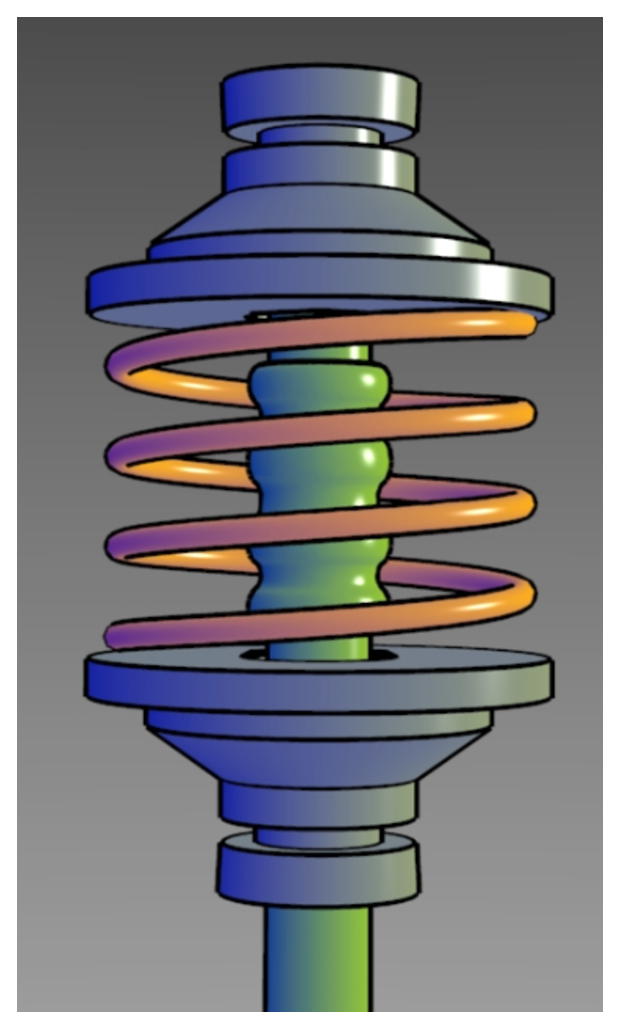
\includegraphics[scale=0.5]{techreview_v1/one.eps}
  \caption
{ \newline \hspace{\linewidth}
Gooch shaded model showing the implementation of black edge lines combined with curve highlights and warm to cool hue shifts.}
  \label{fig:one}
\end{figure}

\paragraph{Cel Shading}
A common type of non photorealistic shading that is primarily used to give 3D objects in computer graphics a flat, 2D look. 
It accomplishes this by using fewer shading colors as opposed to the traditional shading gradient
Additionally, in cel shading, color hues are distinct and do not blend. \cite{celshading}
This is implemented by defining constant light intensities at certain regions and is responsible for the main visual difference between realistic shading and cel shading. 
The lighting in cel shading is done per pixel and can be implemented in either the vertex or fragment shader. \cite{nonphotshading} 
Figure 2 below illustrates the differences between cel and realistic shading.

\begin{figure} [H]
  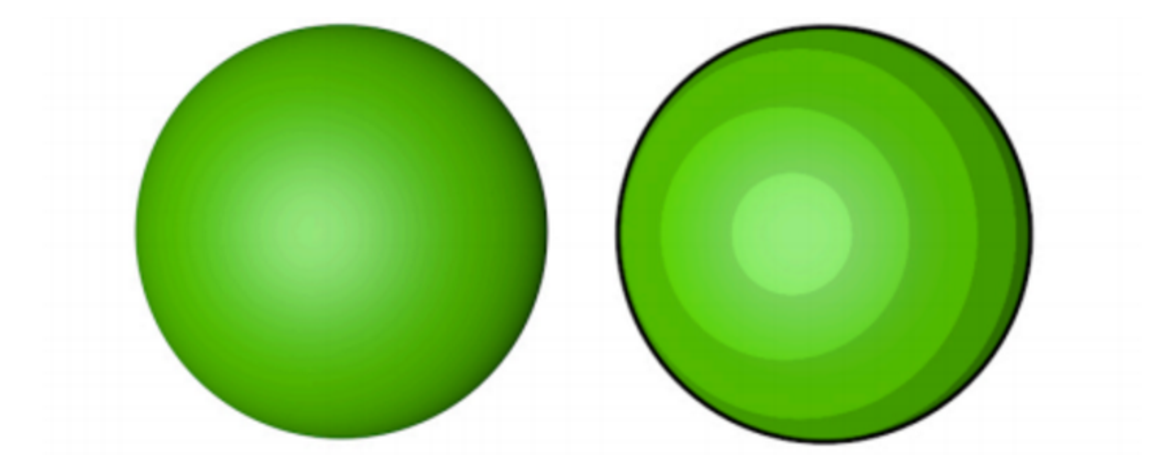
\includegraphics[scale=0.5]{techreview_v1/two.eps}
  \caption
{ \newline \hspace{\linewidth}
On the left is an object shaded using realistic shading. 
Observe that there is a wide range of shading colors and that colors blend together. 
On the right is an object shaded using cel shading.
Notice that color hues are few in number and are distinct from each other (I.E. do not blend).}
  \label{fig:two}
\end{figure}

\paragraph{Hatching}
A non photorealistic shading technique that does shading by drawing multiple hatches (parallel lines) to highlight darker parts of an object. 
The general rule of thumb is the darker the area, the more hatches are drawn there. 
The length, width, and distance between hatches are defined by the developer.
If the hatches are not parallel and instead cross, then it is called cross-hatching. \cite{hatch}
Drawing hatches with different angles can help with emphasizing curves in an object.
To implement hatching, textures of different levels of hatching are first created. 
After that, these texture can then be sent to the fragment shader and be assigned based on the lighting of the object.
Figure 3 what a 3D cat would look like if it was shaded using hatching.

\begin{figure} [H]
  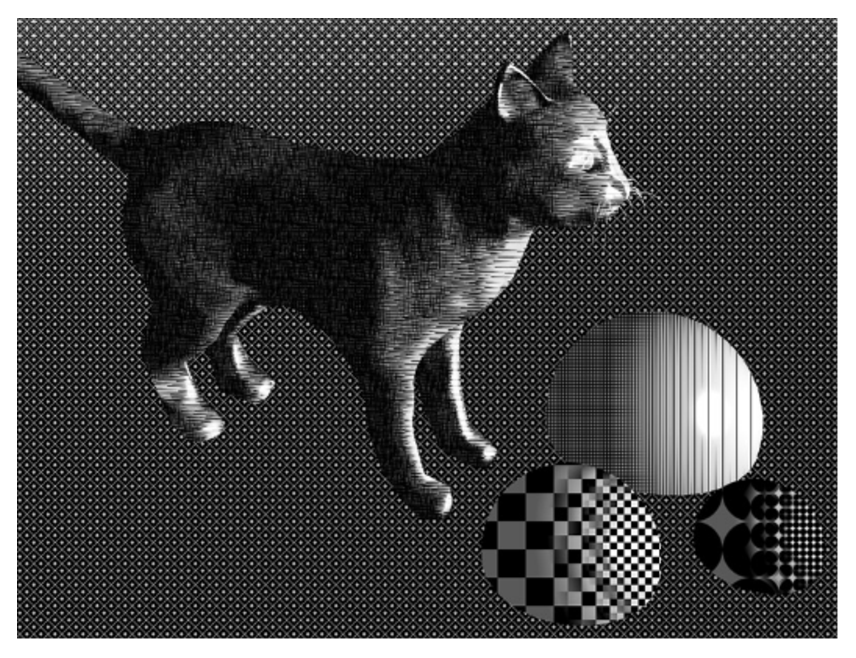
\includegraphics[scale=0.5]{techreview_v1/three.eps}
  \caption
{ \newline \hspace{\linewidth}
3D cat drawn using simple hatching. Notice that the number of hatches drawn is used to highlight the curves of the cat and is based on the light position.}
  \label{fig:three}
\end{figure}

\paragraph{Goals}
Our client wants the shading to primarily highlight object shape. 
This entails focus on emphasizing the curves of objects, 
They also want all parts of any 3D rendered object to be visible if it is within view.
This would mean that no piece of an object should be completely black as this would possible confuse the object's shape.

\paragraph{Criteria}
These technologies will be primarily judged based on how well they highlight object shape and visibility. 
Additionally, how well each are documented will be considered.
Speed, resource cost, and implementation flexibility will also be factored in but at a lower priority. 
This is because the speed and cost of shading implementations are more dependent on the specific implementation rather than the type of shading.

\paragraph{Table}
\begin{center}
\begin{table}[H]
\begin{tabular}{ | m{7em} | m{7em} | m{7em} | m{7em} | m{7em} | m{7em} |  } 
\hline
\textbf{Technology}  & \textbf{Highlight Shape} & \textbf{Object Visibility} & \textbf{Documentation} & \textbf{Speed \& Cost} & \textbf{Flexibility} \\ \hline
Gooch Shading & Shape highlighted using warm to cool colors tones. & No parts of the 3D object is completely blacked out. & Well documented. Original paper detailing Gooch Shading available online. & Uses equations to calculate tones of a color. Will mostly depend on specific implementation. & Can be implemented with fragment or vertex shader.  \\ \hline
Cel Shading & Shape highlighted using few shading colors. Color hues do not blend which creates a 2D look for the shape. & Object areas have constant light intensities so they aren't typically completely black. & Widely used and well documented. Many pieces of sample code exist online. & Fast and efficient due to fewer shading colors and constant light intensities. & Lighting can be done using vertex or fragment shader.  \\ \hline
Hatching & Shape highlighted by using textures with different number of hatches. The darker the area, the more hatches. & Darker areas of an object have more hatches drawn there meaning parts of it could be completely black. & Not as common as cel or Gooch shading but documentation still exists. & Depends on implementation. Hatches typically drawn using textures and lighting equations. & Must use both vertex and fragment shader. \\ \hline
\end{tabular}
\newline
\caption{Comparing non photorealistic shading technologies}
\label{table:nonphoto}
\end{table}
\end{center}

\newpage

\paragraph{Discussion}
All three shaders do well at highlighting object shape. 
For our purposes, however, Gooch shading and Hatching do a better job since they allow for the object to retain its 3D shape. 
Cel shading makes objects look 2D which, for us, is bad.
Gooch and cel shading both do well at keeping full object visibility. 
Hatching has the possibility of completely blackening certain parts of objects which means visibility may be a problem.
Cel shading is the most well documented since it is the most common type among the 3. 
Gooch is not far behind with its documentation widely available online.
Hatching is the least well documented, but resources still exist online.
Cel is likely the fastest and most efficient among the 3 shaders but the others aren't far behind.
Gooch and cel shading can be implemented using either the vertex or fragment shader while Hatching must use both.
This is not much of a problem, however, since our implementation will likely use both anyways.

\paragraph{Choice}
For our purposes, Gooch shading is the best option. 
It does a great job at highlighting object shape while also guaranteeing full object visibility. 
Additionally, good documentation exists online for it so getting started won't be an issue.
The other two types of shading weren't selected because they didn't highlight both object shape and visibility.
Cel doesn't do well at highlighting 3D curves and Hatching does a poor job at showing object visibility.

\newpage

\subsubsection{Silhouettes}

\paragraph{Stencil Buffer Technique}
Technique for rendering a silhouette edge around a 3D object using the stencil buffer.
This technique can draw the silhouette of an object before or after the object is drawn.
In this algorithm, the object is drawn 4 times; each time displaced by 1 pixel in the x or y direction. \cite{silhouette}
This offset is done in windows coordinates and can be implemented by changing the viewport coordinates each time.
The algorithm, in detail, is provided below [6]:
\begin{enumerate}
\item If you want to see the object itself, render it in the usual way.
\item Clear the stencil buffer to zero.
\item Disable writing to the color and depth buffers
\item Set the stencil function to always pass, set the stencil operation to increment
\item Translate the object by +1 pixel in y, using glViewport()
\item Render the object
\item Translate the object by -2 pixels in y, using glViewport()
\item Render the object
\item Translate by +1 pixel x and +1 pixel in y
\item Render
\item Translate by -2 pixel in x
\item Render
\item Translate by +1 pixel in x. You should be back to the original position.
\item Turn on the color and depth buffer
\item Set the stencil function to pass if the stencil value is 2 or 3. Since the possible values range from 0 to 4, the stencil function can pass if stencil bit 1 is set (counting from 0).
\item Rendering any primitive that covers the object will draw only the pixels of the silhouette. For a solid color silhouette, render a polygon of the color desired over the object [6].
\end{enumerate}

\newpage

\paragraph{Silhouettes using Polygonal offsets}
A common technique to draw silhouettes often used in cel shading (note cel shading itself not necessary to use this technique).
To implement these silhouettes, first render an enlarged version of the object with a constant color (black). \cite{nonphotorealisticsilhouette}
After that, render the object again but with its normal size and a different color over the top of the enlarged version.
This process is shown visually in Figure 4 below:

\begin{figure} [H]
  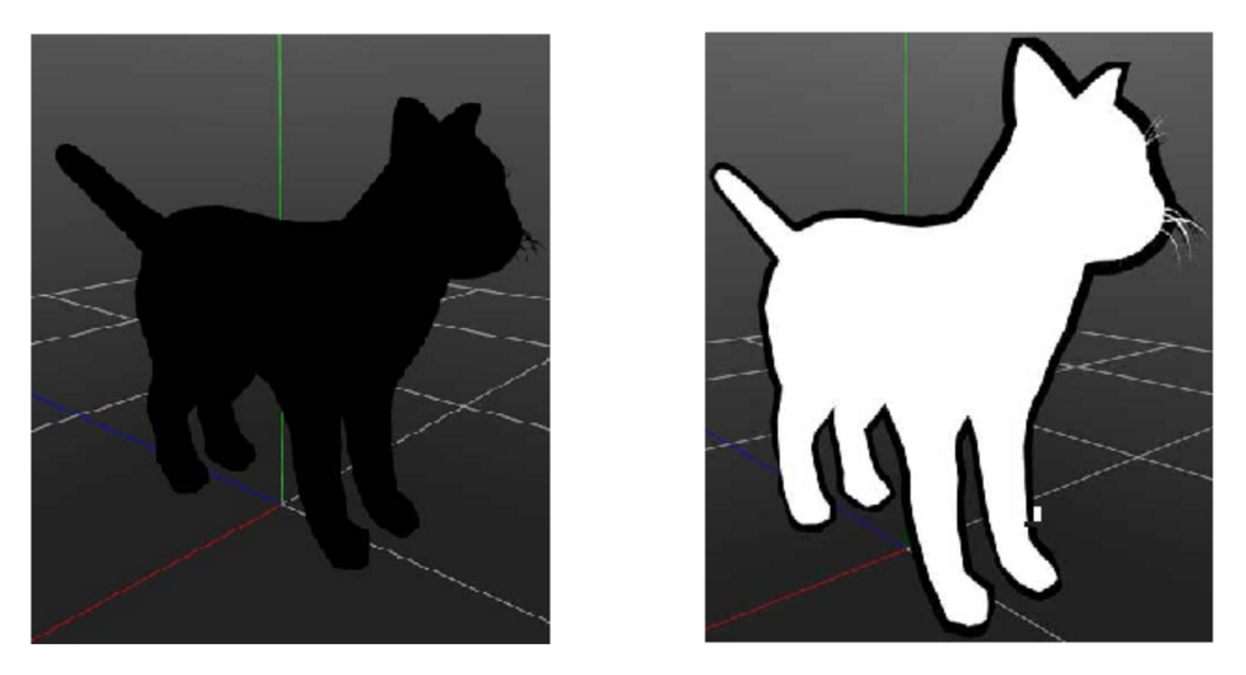
\includegraphics[scale=0.5]{techreview_v1/four.eps}
  \caption
{ \newline \hspace{\linewidth}
On the left is the scene after the first rendering. The scene displays an enlarged version of the object drawn only in black. On the right is the scene after the second rendering. The second rendering draws the object (in white) with its normal size over the enlarged version creating the silhouette.}
  \label{fig:four}
\end{figure}

\paragraph{Edge Detection Silhouettes}
The basic idea of this technique is find all the front facing edges of the object and to place them in a list.
There are multiple algorithms out there to do this such as the Frei-Chen edge detection algorithm. \cite{edgedetector}
After the edge list is created, draw along the list in black (or any other desired color) and the silhouette will be drawn. \cite{toonshading}
The main part of this technique is the edge detection. 
Although multiple algorithms exist, some are exceedingly slow and others are difficult to implement.

\paragraph{Goals}
Silhouettes should define an object's borders. 
In other words, they define where an object begins and ends.
Their primary purpose is to help differentiate objects in the scene from each other.
This will assist in defining an object's position within the scene.

\paragraph{Criteria}
These silhouettes will be judged on smoothness, ease of implementation, efficiency, flexibility, and how well documented it is.
Smoothness is self explanatory; silhouettes should not appear jagged when zoomed in on.
Ease of implementation varies greatly between different silhouette techniques; implementation time should only be increased if the benefit is significant.
Efficiency will be determined by how the silhouette is created. Some techniques create it by drawing the object twice, others create it by traversing the object's vertices.
Flexibility is measured by how the silhouette behaves under different situations. For example, does it work when objects overlap?

\paragraph{Table}
\begin{center}
\begin{table}[H]
\begin{tabular}{ | m{7em} | m{7em} | m{7em} | m{7em} | m{7em} | m{7em} |  } 
\hline
\textbf{Technology}  & \textbf{Smoothness} & \textbf{Implementation Difficulty} & \textbf{Efficiency} & \textbf{Flexibility} & \textbf{Documentation} \\ \hline
Stencil Buffer Technique & Based on how the original object was drawn since its vertices to create the silhouette. & Involves messing with the Stencil Buffer. Algorithm to implement these silhouettes provided online. & Draws the object 4 times. & Handles overlapping objects well. It can display just silhouette edges or edges and borders. & Well documented on OpenGL websites and other sources.  \\ \hline
Polygonal offset & Based on how the original object was drawn since its vertices to create the silhouette. & Easy. Simply draw the object twice but with an offset on one of them. & Draws the at least twice. & Struggles when objects overlap since the silhouette is a background object. & Well document since it is easy to implement and commonly used in cel shading.  \\ \hline
Edge Detection & Based on how the original object was drawn since its vertices to create the silhouette. & Varies depending on the edge detection algorithm used. & Traverse through every vertex of the object. Efficiency also dependent on edge detection algorithm. & Handles overlapping objects well since separate objects have their own edge lists. & Not well documented. Resources mostly come from forum posts and stackoverflow questions. \\ \hline
\end{tabular}
\newline
\caption{Comparing silhouettes technologies}
\label{table:silhouettes}
\end{table}
\end{center}

\newpage

\paragraph{Discussion}
All three silhouette drawing methods have the ability to create smooth silhouettes since they are all based on how the object was drawn.
The polygonal offset method is by far the easiest to implement since it is just drawing the object twice but with an offset.
The stencil buffer technique has a detailed and clear algorithm for its implementation so it's simple to implement too.
The edge detection method is less clear due to lack of solid documentation.
The polygonal offset and edge detection methods are similar in efficiency while the stencil buffer technique is the most inefficient (since it has to draw the object four times).
The only method that struggles with overlapping objects is the polygonal offset method. 
This is significant since overlapping objects are common in 3D scenes.
All three methods have resources online, but the edge detection method is the least well documented.

\paragraph{Choice}
The stencil buffer technique is the best method for our purposes.
It is well documented so implementing it will be straightforward.
Additionally, it is flexible in what it displays (silhouette edges, borders, etc.) and when it is applied (after object is drawn or before). 
The only draw back is its efficiency since it has to draw the object four times.
There are, however, modifications to the algorithm that can reduce the number of times it has to draw to two. \cite{siledges}
The edge detection case was not chosen because it is not well documented.
The polygonal offset choice, while easy to implement and well documented, was not chosen because it lacked flexibility.

\newpage

\subsubsection{Optimization - Run time analysis}

\paragraph{CodeXL}
A powerful OpenGL and OpenGL ES debugger that was once called gDEBugger before it was bought out by AMD.
It traces application activity on the OpenGL API which will assist with finding bugs and boosting performance.
CodeXL can be applied to a variety of applications and works on Windows and Linux platforms.
Using it is as simple as just running the application in the debugger.
Additionally, CodeXL has a multitude of features that will assist in the debugging process such as static shaders analysis, GPU profiling, and power profiling. \cite{codexl}
CodeXL is available on github and is free to use.

\paragraph{GLSL-Debugger}
An open source fork of the glslDevil project.
GLSL-Debugger is a tool for debugging OpenGL programs.
Key features include tracing OpenGL programs, visual GLSL step-by-step debugging, support for Linux and Windows, and record and playback OpenGL traces [11].
The source code is available online for free but requires the user to compile it.
Instructions for how to do this is shown on their website.

\paragraph{GLIntercept}
GLIntercept is a OpenGL function call interceptor available for the windows platform. \cite{glsl}
To use it, user must copy certain install files (opengl32.dll and a gliConfig.ini) to the executable folder and then edit the gliConfig.ini file to their liking.
Additionally, GLIntercept has a variety of feature including function call logging, saving and tracking of shaders, saving and tracking of display lists, function stats, and more.
GLIntercept is available on github for free.
Importantly note that this debugger may not work on advanced features in OpenGL 3.0+ due to it being developed using the OpenGL 1.0-2.1 debugger [12].

\paragraph{Goals}
The goal of this runtime analyzer is to improve application performance by tracing where resources are being used in the program.
In general, our modifications should not slow down the current implementation as that would hurt the smoothness of the simulation.
This analyzer will help track the changes our modifications are making to the program.

\paragraph{Criteria}
The debuggers will be judged based on relevant features, usability, and documentation.
Relevant features include function call tracing, data structure tracking, available platforms, etc.
Usability is measured by how easy it is to install and use.
Documentation is measured by how many resources on the debugger are available online.
The first two factors will be of higher priority than the third because not having certain features is much more important than amount of documentation.

\paragraph{Table}
\begin{center}
\begin{table}[H]
\begin{tabular}{ | m{7em} | m{7em} | m{7em} | m{7em} | m{7em} | m{7em} |  } 
\hline
\textbf{Technology}  & \textbf{Program tracing and tracking} & \textbf{Other Relevant Features} & \textbf{Usability} & \textbf{Available Platforms} & \textbf{Documentation} \\ \hline
CodeXL & Included  & Static Shader Analysis. GPU and Power profiling. & Easy to use and download. Quick start guide available for download.
Uses a GUI to display resource consumption. & Windows and Linux. & Well documented with a quick start guide available.  \\ \hline
GLSL\-Debugger & Included & None & Source code available online. Must build and compile yourself. Uses a GUI to display program tracing. & Windows and Linux. & Not very well documented. Their website has enough documentation to get the debugger built.  \\ \hline
GLIntercept & Included & Resource leak tracing, tracking of error states, function timer logs. & Source code available online. Must copy files over and edit certain files to debug. No GUI. & Windows. & Well documented. Github page has detailed list of features and short tutorial on how to use it. \\ \hline
\end{tabular}
\newline
\caption{Comparing run time analysis technologies}
\label{table:runtime}
\end{table}
\end{center}

\newpage

\paragraph{Discussion}
As far as features go, all of the debugger have the minimum necessary features to warrant use (I.E. program tracing).
CodeXL has the most available features, but they may not all be useful to us.
GLSL-Debugger has the fewest features while GLIntercept is somewhere in the middle.
In the usability department, CodeXL ends up on top.
It's not only easy to install, but it also comes with a useful GUI for debugging.
GLSL-Debugger also comes with a GUI, but it is trickier to get working.
GLIntercept has no GUI which hurts its overall usability.
For available platforms, the only debugger that doesn't work on Linux is GLIntercept.
This is significant as it factors into other parts of our project such as maintenance.
When it comes to documentation, CodeXL once again comes out on top.
Its provided quick start guide shows useful examples on how to install and use the application.
GLIntercept has good documentation, but no examples while GLSL-Debugger only provides screenshot for how to use it.

\paragraph{Choice}
CodeXL is the best debugger for our purposes.
It provides many useful features for us to use while also being user friendly. 
Additionally, good documentation for it is available online; the aforementioned quick start guide is especially useful.
The GLIntercept debugger was not chosen because it was limited on platform.
The project must work on Linux so having a debugger that doesn't work on Linux would be a hassle.
GLSL-Debugger was not chosen because it was too simple (in terms of features) and not very well documented.

\newpage

\subsection{Usability inspection methods, Using the selected inspection method, and Data Analysis Tools}
\large{By Daniel Goh}

\normalsize
\subsubsection{Usability Inspection Methods}
Usability inspection will be carried out to measure the improvement between the starting and the end phase of the project.
Usability.gov lists multiple usability inspection methods that can be used to determine the usability of an interface. \cite{userResearch}
The three main inspection methods that suits this project scope include: Individual Interviews, Online Surveys, and System Usability Scale (SUS).
This section will be used to review various inspection methods and select one that will best suit this project.

\paragraph{Individual Interviews}
An individual interview is an inspection method in which a interviewer talks to the participant for 30 minutes to an hour.
During this interview, the interviewer is tasked to gain a deeper understanding of the participants.
This includes taking note of the participant's attitudes, beliefs, desires, and experiences.

Guidelines to conduct individual interviews as defined by usability.gov are as follows:
\begin{itemize}
\item Define the aim of the study and select relevant participants.
\item Prepare interview protocol which includes questions and probes to use during the interview.
\item Create a comfortable interview situation by asking questions in a neutral manner and be attentive for probe queues.
\item Get permission to tape interview session, and have one or more note takers during the interview.
\end{itemize}

Benefits of Individual Interviews:
\begin{itemize}
\item Researchers will be able to gain a better understanding of individual participants.
\item Researchers will be able to observe the participant's body language and facial emotions during the interview.
\item Researchers will be able to receive additional insights that might not have occurred to the interviewer.
\end{itemize}

\paragraph{Online Surveys} 
An online survey is a form of feedback that is done over the internet.
This inspection method is structured as a questionnaire, and is published online to gather feedback from a broad audience.
The data is then stored within a database, and a survey tool is used to analyze the data.

Guidelines to conduct individual interviews as defined by usability.gov are as follows:
\begin{itemize}
\item Identify purpose of the survey.
\item Determine and select target audience that will best suit the project.
\item Identify methods to collect data and limitations to data collection.
\item Create brief surveys.
\item Provide estimated time to completion up front, and show progress of survey to participants.
\item Mix in open-ended questions with closed questions.
\item Allow participants to choose to answer in-depth questions through a follow-up session.
\end{itemize}

Benefits of Online Surveys:
\begin{itemize}
\item Researchers will be able to reach to a broader audience.
\item Researchers will be able to learn who the users are.
\item Users will be more willing to participate as it would not take up too much time.
\item A wide variety of survey tools are available online.
\item Cost efficient for researchers.
\end{itemize}

\paragraph{The System Usability Scale} 
The System Usability Scale (SUS) is a tool created by John Brooke in 1986.
The SUS method is structured as a ten item questionnaire that requires users to rate individual items with five response options; from Strongly agree to Strongly disagree.

Guidelines to conduct System Usability Scale as defined by usability.gov and UsabilityNet.org are as follows:
\begin{itemize}
\item Participants should not spend time thinking about items for a long time, instead they should record their immediate response. \cite{usabilitynet}
\item The questionnaire are defined and covers the need for support, training, and complexity of system usability.
\item Data gathered through this method needs to be "normalized" to produce a percentile ranking.
\end{itemize}

Benefits of The System Usability Scale:
\begin{itemize}
\item Easy to scale to administer to participants.
\item Study can yield reliable results, even on small sample sizes
\item The System Usability Scale is an industry standard, and is credible in differentiating usable systems from unusable ones.
\end{itemize}

\paragraph{Goals}
The goals of running usability inspections is used to determine if our team was able to successfully improve the current simulation's visuals.

\paragraph{Criteria}
The criteria of selecting a suitable usability inspection method is as follows:
\begin{itemize}
\item Needs to easily allow participants to view and choose between two pictures (old visualization and new visualization)
\item Needs to allow the team to get at least 20 respondents within 6 weeks
\item Needs to take less than 10 minutes of the participants time to increase participation willingness
\end{itemize}

\paragraph{Table}
\begin{center}
\begin{table}[H]
\begin{tabular}{ | m{10em} | m{15em} | m{15em} | m{15em} |  } 
\hline
\textbf{Methods}  & \textbf{Time needed of team to conduct method per session} & \textbf{Time needed of participant to participate} & \textbf{Estimated amount of people that can be reached within 6 weeks} \\ \hline
User Interview & approx. 30 minutes  & approx. 30 minutes & approx. 20 people \\ \hline
Online Survey & None & approx. 5 minutes & approx. 50 people \\ \hline
System Usability Scale & approx. 10 minutes & approx. 10 minutes  &  approx. 50 people \\ \hline 
\end{tabular}
\newline
\caption{Comparing the efficiency between user interviews, online surveys and using the System Usability Scale}
\label{table:inpectionmethods}
\end{table}
\end{center}

\paragraph{Discussion}
All three listed usability inspection methods are widely adopted inspection methods.
Individual interviews would allow the team to better understand the participant's wants and thoughts, however it would require more time from the participant and the conductor of the interview.
Online surveys would allow the team to get data with less work required for the team and the participants.
However, the team would not be able to get additional body language queues without observing the participants directly.
The System Usability Scale, a questionnaire like inspection method would allow the team to gather data about the simulation as a whole, however that is not within the scope of the project assigned by the client.

\paragraph{Choice}
After reviewing the available usability inspection methods, the \textbf{online survey method} would be a better fit for our project.
By utilizing online surveys, the project would be able to collect more insight from a larger and broader audience.
Individual interviews would not be appropriate as our project does not require an emotional understanding of the participant's thoughts and body language.
The System Usability Scale employs questions that dives too deep into the system, and would introduce scope creep in comparison to the requirements provided by our client.
Thus, the \textbf{online survey method} will be utilized as a usability inspection method to measure the success of the project.

\newpage

\subsubsection{How to carry out selected inspection method: Online Surveys}
There are many survey tools available online.
This section reviews the various survey tools that are free to use.
The reviews are done after using the survey tools first-handedly.

\paragraph{Google Forms}
This section covers the pros and cons of Google's survey tool, Google Forms.

Pros of Google Forms for our project purpose:
\begin{itemize}
\item Allows unlimited questions in a form
\item Collected data are visualized as pie charts
\item Collected data can be exported into Google Spreadsheets (Google's equivalent of Microsoft Excel)
\item Collected data can be exported as a .csv file to be use with other data analysis tools
\item Allows images and videos to be added into each survey questions without the need to host them externally
\item Allows unlimited respondents to take the survey
\end{itemize}

Cons of Google Forms for our project purpose:
\begin{itemize}
\item As the collected data are stored on Google's remote servers, we are giving Google (and their affiliated partners) "a worldwide license to use, host. store, reproduce, create derivative works, communicate, publish, publicly perform, publicly display and distribute" the content \cite{google}
\end{itemize}

\paragraph{Survey Monkey}
This section covers the pros and cons of Survey Monkey.

Pros of Survey Monkey for our project purpose:
\begin{itemize}
\item Well known as an online survey tool
\item Contains a variety of different questions types
\item Has a dedicated "SurveyMonkey and IRB Guidelines" under the policies section
\item Provides assistance with IRB approvals by providing "evidence permission to use the SurveyMonkey platform to conduct research" \cite{surveymonkey}
\end{itemize}

Cons of Survey Monkey for our project purpose:
\begin{itemize}
\item Only allows 10 questions
\item Only allows 100 respondents
\item No data export capability
\item No data reporting capability
\end{itemize}

\paragraph{Typeform}
This section covers the pros and cons of Typeform.

Pros of Typeform for our project purpose:
\begin{itemize}
\item Allows unlimited questions
\item Allows unlimited respondents
\item Supports data export
\item Respondent's input can be piped into other questions (User inputs their name for the first question, and the second question can access their name and call them by name in upcoming questions)
\item Interface is modern and beautifully designed
\end{itemize}

Cons of Typeform for our project purpose:
\begin{itemize}
\item Uses keyboard as main input for survey questions
\end{itemize}

\paragraph{Goals}
The goal of selecting a survey tool is to allow the team to carry out the online survey inspection method as efficiently as possible.

\paragraph{Criteria}
The criteria of selecting a suitable online survey platform is as follows:
\begin{itemize}
\item Needs to be free to use
\item Needs to easily allow participants to view and choose between two pictures (old visualization and new visualization)
\item Needs to allow participants to complete the survey across multiple device platforms with an integrated browser (e.g. Internet Explorer for Windows, Safari for macOS and iOS devices etc.)
\item Needs to allow data export for data analysis
\item Needs to allow at least 10 questions to be asked
\end{itemize}

\paragraph{Table}
\begin{center}
\begin{table}[H]
\begin{tabular}{ | m{10em} | m{15em} | m{15em} | m{15em} |  } 
\hline
\textbf{Tools}  & \textbf{Image integration} & \textbf{Data export support} & \textbf{Number of questions allowed} \\ \hline
Google Forms & Included  & Supports Google Sheets, .xlsx, .ods, .tsv and .csv export & Unlimited \\ \hline
Survey Monkey & Included & Supports .xls, .xlsx, Google Sheets, .spss and .csv export & 10 \\ \hline
Typeform & Included & Supports .xlsx and .csv export &  Unlimited \\ \hline 
\end{tabular}
\newline
\caption{Comparing the survey tool features provided in Google Sheets, Survey Monkey and Typeform}
\label{table:surveytool}
\end{table}
\end{center}

\newpage

\paragraph{Discussion}
All three listed survey tools are commonly used in both professional and non-professional settings.
Google Forms and TypeForm allows unlimited questions, and does not limit the number of respondents.
However, Google Forms supports the most data export option as Google Forms is tightly integrated with Google Sheets, which allows various sheet export options.
Survey Monkey offers a simpler version for free from it's paid counterpart.
The free version only allows 10 questions and 100 respondents in the free version, and this might pose to be an issue if the team decides to increase the number of questions in the survey.
Similar to Survey Monkey, Typeform is a survey tool that offers free and PRO tiers based on the needs of the survey.
Both Survey Monkey's and Typeforms' premium offerings (Logic jumps, priority customer support) are not vital for the survey.

\paragraph{Choice}
After reviewing various survey tools, \textbf{Google Forms} comes in as the best choice that fits the selected usability inspection method.
Our survey will not collect sensitive information (e.g. social security numbers, credit card numbers etc.), thus it is safe if Google make the data accessible to the public.
The purpose of the survey (to compare the simulation visuals prior to enhancement and after enhancement) is unrelated to the original research, and does not need to be kept confidential.

\newpage

\subsubsection{Data analysis tools to analyze and visualize collected data}
Data analysis and visualization tools are used in enterprise situations to allow massive data to be processed into meaningful data.
With the inspection method and survey tools selected, a suitable data analysis and visualization tool will be needed to process the raw data.
As the selected survey tool allows csv (comma separated value files) to be exported, the review will only include tools that can process csv files and that are free of charge.
The reviews for data analysis and visualization tools are done after using the applications first-handedly. 

\paragraph{Google Forms, Google Sheets}
Google has a wide range of applications in their portfolio, and the survey tool selected, Google Forms come with an integrated pie chart visualizer.
However, users will be able to transfer the survey data into Google Sheets for a more complete data analysis environment.

Pros of using Google's visualization for our project purpose:
\begin{itemize}
\item Easily transferable across Google platforms
\item Easily shared across multiple collaborators
\item Simple, light weight and easy to use
\item Work can be done in a web browser
\item Keeps records of previous spreadsheet versions for reverting purposes
\end{itemize}

Cons of using Google's visualization for our project purpose:
\begin{itemize}
\item Limited chart types
\item Google (and their affiliated partners) is given "a worldwide license to use, host. store, reproduce, create derivative works, communicate, publish, publicly perform, publicly display and distribute" the content \cite{google}
\end{itemize}

\paragraph{Microsoft Excel}
Microsoft Excel is an application that requires a subscription fee (as a part of Office 365) to access.
However, as an Oregon State University student, we have access to use the software with a student license.
Microsoft Excel is the leader of all spreadsheet applications.

Pros of using Microsoft Excel for our project purpose:
\begin{itemize}
\item Easy to create charts from CSV files
\item Contains many chart customization options
\item Allows the user to manipulate and show the data in many different ways through PivotCharts
\end{itemize}

Cons of using Microsoft Excel for our project purpose:
\begin{itemize}
\item History keeping of excel files are not reliable
\item PivotCharts requires user overhead to correctly manipulate
\end{itemize}

\paragraph{d3.js}
D3.js is a JavaScript library that is used to manipulate documents based on the data that is fed into it.
D3 emphasizes it's output on web standards, and only requires an internet browser to show the visualization of data.

Pros of using D3.js for our project purpose:
\begin{itemize}
\item Contains many beautifully designed templates that can be used
\item Code base is open sourced
\item Can display dynamic visualization on web pages
\item Visualization updates on the fly as data gets updated
\end{itemize}

Cons of using D3.js for our project purpose:
\begin{itemize}
\item Not a thorough data analysis tool, but mainly a data visualization tool
\item Has a steep learning curve to get things running
\end{itemize}

\paragraph{Goals}
The goal of selecting a good data analyzer/visualizer tool is allow the team to analyze and visualize data collected from the survey.
This should be done in the most efficient manner without sacrificing the quality of the analyzed data and data visualization.

\paragraph{Criteria}
The criteria of selecting a data analysis/visualizer tool is as follows:
\begin{itemize}
\item Needs to be free to use
\item Needs to read .csv data files
\item Needs to be supported across different operating systems
\end{itemize}

\paragraph{Table}
\begin{center}
\begin{table}[H]
\begin{tabular}{ | m{10em} | m{15em} | m{15em} | m{15em} |  } 
\hline
\textbf{Tools}  & \textbf{Reads .csv files } & \textbf{Documentations} & \textbf{Cloud editing} \\ \hline
Google Sheets & Yes  & Yes (Moderately detailed) & Yes \\ \hline
Microsoft Excel & Yes & Yes (Very detailed) & Yes \\ \hline
D3.js & Yes & Yes (Moderately detailed) & No \\ \hline 
\end{tabular}
\newline
\caption{Comparing the features between Google Sheets, Microsoft Excel and D3.js}
\label{table:datatools}
\end{table}
\end{center}

\newpage

\paragraph{Discussion}
All three listed data analysis/visualizer tools are the more commonly used tools available.
All three tools supports .csv file importing.
Google Sheets and Microsoft Excel (Office 365) allow cloud editing, this provides the team the convenience of accessing the data anywhere.
With cloud editing, comes cloud backup.
Both Google Sheets and Microsoft Excel (Office 365) backs up the data file periodically.
This allows easy recovery from unforeseen circumstances.
Both Microsoft Excel and D3.js offer various type of chart and visualization support, whereas Google Sheets only carries a limited number of chart types.
However, the chart type variants does not have a significant impact on the tool choice as the provided charts within Google Sheets accommodates the conventional chart types.

\paragraph{Choice}
After reviewing the different data analysis and visualization tools, \textbf{Google Sheets} will be used for data analysis and visualization purposes.
As many of the project documents reside in a collaborative Google Drive, migrating the data analysis portion out from a well constructed ecosystem is not necessary.
With Google Sheets, the spreadsheet can be worked on collaboratively and can be shared with the client for better transparency on the ongoing data analysis. 

\newpage

\subsubsection{Conclusion}
In conclusion, debugging techniques will be used to identify the render loop.
Refactoring code will assist code maintainability.
The shadow volume implementation will be used to implement shadows.
Gooch shading will be implemented for non photorealistic shading.
The stencil buffer technique will be used to implement silhouettes.
CodeXL will be used for run time analysis.
Online surveys will be used to carry out usability inspection.
Google Forms will be used to carry out the online survey.
And Google Sheets will be used to do the data analysis and visualization.

\bibliographystyle{IEEEtran}
\bibliography{techreview}

\section{Tech Review Update}

\begin{center}
\begin{table}[H]
\caption{Table showing the technology that is changed (Technology), what happened to it (Change Details), and comments for the change(Comments).}
\begin{tabular}{ | p{0.2\linewidth} | p{0.2\linewidth} | p{0.5\linewidth} | }
\hline
\textbf{Technology}  & \textbf{Change Details}  & \textbf{Comments} \\ \hline

Shading Method & 
Technology did not change (still uses Warm Cool shading), only implementation. & 
As stated in the design doc., now adapts to the object's original color and is now implemented using the SoShadowGroup library. \\ \hline
Silhouettes &
Now uses GL\_LINES method instead of the silhouette edge algorithm. &
The silhouette edge algorithm required direct control over some OpenGL tools (like the view port and the depth buffer) that we did not have access to.
The GL\_LINES method was chosen because it has consistent silhouette widths throughout objects (cel shaded silhouettes did not). \\ \hline
Debugger  &
Went from CodeXL to testing using multiple machines to render the scene. &
Firstly, as stated in the design doc. table, CodeXL only works on Windows while our system runs on Ubuntu 16.04 so we can not even use it.
Secondly, it's easier to test and debug this system by running the simulations on different computers and then examining the scene.
Lastly, the fps requirement was removed in our requirements document so optimization was not a focus. \\ \hline
Survey Platform  &
Platform to run survey was switched from Google Forms to Qualtrics. &
Oregon State University provides Qualtrics license to its students, which allows us to utilize the premium features provided.
This platform allows us to enhance the survey's design and customization. \\ \hline
Data Analysis and Visualization Tool &
Data analysis and visualization tool switched from Google Sheets to Qualtrics' built-in data analysis and visualization tools. &
Qualtrics' built-in features allow direct data analysis and visualization, allowing more efficient data reporting. \\ \hline
Code Maintainability &
Technology did not change. &
We continued to use version control and documentation throughout the project to ensure that our code was protected and easily changeable for future programmers. \\ \hline
Shadows &
Technology changed to variance shadow mapping. &
This technology changed from the shadow volume implementation.
It turned out it would be extremely difficult to create our own shadows, and there was already a built in shadows class that we could us for shadows. \\ \hline


\end{tabular}
\newline
\label{table:TechReviewUpdate}
\end{table}
\end{center}

\newpage

\section{Weekly Blog Posts}
\subsection{Fall 2016}

{\setstretch{1.0}
\subsubsection{Week 4}
\paragraph{Justin Bibler}
\subparagraph{Plans for next week}
\begin{itemize}
  \item 10/24 Participate in the simulation study.
  \item Get signature, and have our problem statement signed.
  \item Review IEEE standard.
  \item Write requirements document.
  \item Develop team name.
\end{itemize}

\subparagraph{Progress made this week}
\begin{itemize}
  \item Revised problem statement, based on feedback.
\end{itemize}

\subparagraph{Problems Encountered}
\begin{itemize}
  \item None.
\end{itemize}
\vspace{3mm}

\paragraph{Matt Huang}
\subparagraph{Plans for next week}
\begin{itemize}
  \item Participate in the robotic grasping simulation study on Wednesday, Oct 26th.
  \item Get revised problem statement signed by Cindy (our client).
  \item Write requirements document by Friday, Oct 27th.
\end{itemize}

\subparagraph{Progress made this week}
\begin{itemize}
  \item Revised problem statement based on the feedback Kevin gave us. Changes were made to the abstract and problem sections.
    \begin{itemize}
      \item Abstract - Gave context to the overall project (not just our section).
      \item Problem Section - Added high level context to the problem. I.E. what the simulation was used for.
    \end{itemize}
  \item Looked over IEEE 830 format.
\end{itemize}

\subparagraph{Problems Encountered}
\begin{itemize}
  \item None.
\end{itemize}

\vspace{3mm}
\paragraph{Daniel Goh}
\subparagraph{Plans for next week}
\begin{itemize}
  \item Oct. 25 - Get signature from client (Cindy Grimm) for revised Problem Statement document based on availability.
  \item Oct. 27 - Complete requirements document with the team.
  \item Oct. 28 - Participate in the robotic grasping user study.
\end{itemize}

\subparagraph{Progress made this week}
\begin{itemize}
  \item Oct. 21 - Revised Problem Statement with team per Kevin's feedback.
\end{itemize}

\subparagraph{Problems Encountered}
\begin{itemize}
  \item None.
\end{itemize}

}

\newpage

{\setstretch{1.0}
\subsubsection{Week 5}
\paragraph{Justin Bibler}
\subparagraph{Plans for next week}
\begin{itemize}
  \item Put a lot more into the requirements document.
\end{itemize}

\subparagraph{Progress made this week}
\begin{itemize}
  \item Created rough draft of requirements document.
  \item Revised problem statement.
\end{itemize}

\subparagraph{Problems Encountered}
\begin{itemize}
  \item Our requirements document feels very underwhelming since our project is relatively small.
\end{itemize}

\vspace{3mm}

\paragraph{Matt Huang}
\subparagraph{Plans for next week}
\begin{itemize}
  \item Revise requirement document - expand pretty much every section. Get it signed by Cindy.
  \item Participate in the robot grasping simulation on Nov. 2nd.
\end{itemize}

\subparagraph{Progress made this week}
\begin{itemize}
  \item Created rough draft of requirements document.
  \item Decided on team name (Shady Robots).
  \item Completed problem statement (signed and turned in).
\end{itemize}

\subparagraph{Problems Encountered}
\begin{itemize}
  \item Struggled in starting requirements document. Didn't have enough time to properly expand most sections of it.
  \item Dilruba got sick so Daniel and I weren't able to participate in the study this week.
\end{itemize}

\vspace{3mm}

\paragraph{Daniel Goh}
\subparagraph{Plans for next week}
\begin{itemize}
  \item Nov. 1 - Participate in the robotic grasping user study.
  \item Nov. 3 - Complete requirements document with the team.
  \item Nov. 3 - Get signature from client (Cindy Grimm) for revised Requirements Document based on availability.
\end{itemize}

\subparagraph{Progress made this week}
\begin{itemize}
  \item Oct. 24 - Reviewed IEEE 830-1998 format.
  \item Oct. 25 - Met up with team to discuss requirements document and team name.
  \item Oct. 26 - Created and formatted requirements document to IEEE 830-1998 format.
  \item Oct. 27 - Added rough draft of requirements document.
  \item Oct. 28 - Reformatted requirements document (rough draft) for aesthetic purposes.
  \item Oct. 28 - Dropped off requirements document (rough draft) to KEC 2098.
\end{itemize}

\subparagraph{Problems Encountered}
\begin{itemize}
  \item As our project scope is relatively small in scale, it was difficult to flesh out our requirements document based on the IEEE 830-1998 format.
\end{itemize}

}

\newpage

{\setstretch{1.0}
\subsubsection{Week 6}
\paragraph{Justin Bibler}
\subparagraph{Plans for next week}
\begin{itemize}
  \item Review Gooch shading, and Gooch silhouettes.
  \item Start individual tech review.
  \item Revise requirement document, and problem statement further.
\end{itemize}

\subparagraph{Progress made this week}
\begin{itemize}
  \item Revised requirement document, and problem statement.
  \item Got advice for documents from Kirsten Winter, and Nels.
  \item Talked to Mike Bailey for advice on our project.
  \item Received resources to use for shadows from Mike Bailey.
\end{itemize}

\subparagraph{Problems Encountered}
\begin{itemize}
  \item It was difficult to create the requirements document. We thought we didn't have enough content. However, we were able to get help and we'll be able to improve it.
\end{itemize}

\vspace{3mm}

\paragraph{Matt Huang}
\subparagraph{Plans for next week}
\begin{itemize}
  \item Add additional details to requirements doc. I.E. Gooch shading, step by step for shading, longer introduction, etc.
  \item Tech review.
  \item Add additional performance metrics to problem statement.
\end{itemize}

\subparagraph{Progress made this week}
\begin{itemize}
  \item Reviewed and revised most of the problem statement: rewrote abstract and problem summary to only include information relevant to our project.
  \item Finished signed version of requirements doc.
  \item Participated in robot grasping study.
\end{itemize}

\subparagraph{Problems Encountered}
\begin{itemize}
  \item Was difficult to find quantitative performance metrics for graphics.
  \item Was difficult to expand requirements document. Later we got advice from the TA about this.
\end{itemize}

\vspace{3mm}

\paragraph{Daniel Goh}
\subparagraph{Plans for next week}
\begin{itemize}
  \item Nov. 6 - Review Nels' feedback from weekly meeting.
  \item Nov. 7 - Revise Problem Statement with team.
  \item Nov. 7 - Revise Requirements Document with team.
  \item Nov. 8 - Start individual Tech Review document.
\end{itemize}

\subparagraph{Progress made this week}
\begin{itemize}
  \item Nov. 1 - Participate in the robotic grasping user study.
  \item Nov. 2 - Visited Kirsten Winter's office hours with team.
  \item Nov. 2 - Revised introduction of Requirements Document and Problem Statement with team.
  \item Nov. 2 - Added Gantt Chart with team.
  \item Nov. 3 - Revised Requirements Document with team.
  \item Nov. 3 - Drew figure for Requirements Document with team.
  \item Nov. 4 - Revised Requirements Document per client's feedback (Submitted copy).
  \item Nov. 4 - Revised Requirements Document per Nels' feedback during weekly meeting.
\end{itemize}

\subparagraph{Problems Encountered}
\begin{itemize}
  \item (Personal Opinion) Our main problem was to come up with a lengthy requirements document for a project that is small in scope. However, thanks to Nels and Kirsten's guidance, this issue can be solved through a revision of the requirements document.
\end{itemize}

}

\newpage

{\setstretch{1.0}
\subsubsection{Week 7}
\paragraph{Justin Bibler}
\subparagraph{Plans for next week}
\begin{itemize}
  \item Finish Tech Review this weekend.
  \item Continue improving requirements document.
\end{itemize}

\subparagraph{Progress made this week}
\begin{itemize}
  \item Improved requirements document.
  \item Finished revisions on Problem Statement.
\end{itemize}

\subparagraph{Problems Encountered}
\begin{itemize}
  \item None.
\end{itemize}

\vspace{3mm}

\paragraph{Matt Huang}
\subparagraph{Plans for next week}
\begin{itemize}
  \item Finish and turn in Tech. Review. I will be covering and responsible for warm cool shading, silhouettes, and optimization.
  \item Continue to revise requirements document.
  \item Add more details to system features, include user interviews, expand introduction to include client's motivation.
\end{itemize}

\subparagraph{Progress made this week}
\begin{itemize}
  \item Finished editing Problem Statement. Turned it in and got 90/100 on regrade.
  \begin{itemize}
    \item Edits made included rewriting the abstract to fit our scope and changing our performance metric (we're using user interviews now).
  \end{itemize}
  \item Edited requirements document.
  \begin{itemize}
	\item Converted to the modeled shown in Appendix A of the IEEE format.
	\item Added more descriptions on Gooch shading.
	\item Changed how we were citing sources.
  \end{itemize}
\end{itemize}

\subparagraph{Problems Encountered}
\begin{itemize}
  \item None.
\end{itemize}

\vspace{3mm}

\paragraph{Daniel Goh}
\subparagraph{Plans for next week}
\begin{itemize}
  \item Nov. 14 - Turn in Tech Review Document.
  \item Nov. 15 - Revise Requirements Document.
  \item Nov. 15 - Start to draft Preliminary Design Document.
\end{itemize}

\subparagraph{Progress made this week}
\begin{itemize}
  \item Nov. 8 - Revised Problem Statement with team.
  \item Nov. 9 - Revised Requirements Document based on Nels feedback (Issue Tracker).
  \item Nov. 10 - Visited Nels' office hour to get input on Gantt Chart and Tech Review.
\end{itemize}

\subparagraph{Problems Encountered}
\begin{itemize}
  \item None.
\end{itemize}

}

\newpage

{\setstretch{1.0}
\subsubsection{Week 8}
\paragraph{Justin Bibler}
\subparagraph{Plans for next week}
\begin{itemize}
  \item Begin work on design document.
  \item Continue to review over OpenRave source code.
  \item Begin working on progress document.
\end{itemize}

\subparagraph{Progress made this week}
\begin{itemize}
  \item Finished Tech review document.
  \item Reviewed OpenRave source code.
  \item Met with Nels to check up on progress, and receive advice.
\end{itemize}

\subparagraph{Problems Encountered}
\begin{itemize}
  \item Understanding the source code for OpenRave has been a struggle, as there is little documentation.
\end{itemize}

\vspace{3mm}

\paragraph{Matt Huang}
\subparagraph{Plans for next week}
\begin{itemize}
  \item Work on Design Document which is the "how" document.
  \item Work on Progress Report.
  \item If we have time, edit requirements document.
  \begin{itemize}
    \item Need to add online interviews to requirements.
    \item Need to add additional stretch goals.
    \item Need to add details on Gooch shading.
  \end{itemize}
\end{itemize}

\subparagraph{Progress made this week}
\begin{itemize}
  \item Finished technology review.
  \begin{itemize}
    \item Wrote my part on non photorealistic shaders, silhouettes, and runtime analysis.
    \item Met with Daniel to put tech. review together. Ran into organization problems; details included in problems encountered section.
    \item Wrote introduction and conclusion for tech. review.
  \end{itemize}
\end{itemize}

\subparagraph{Problems Encountered}
\begin{itemize}
  \item Problems putting with tech. review.
  \begin{itemize}
    \item Due to communication errors, we all wrote our sections of the tech review differently (in terms of organization).
    \item Some topics weren't quite correct. I.E. we weren't supposed to write about the render loop.
  \end{itemize}
\end{itemize}

\vspace{3mm}

\paragraph{Daniel Goh}
\subparagraph{Plans for next week}
\begin{itemize}
  \item Nov. 20 - Review IEEE Std 1016-2009.
  \item Nov. 21 - Continue drafting of Preliminary Design Document.
  \item Nov. 22 - Meet up with team to work on Design Document.
  \item Nov. 24 - Meet up with team to work on Design Document.
\end{itemize}

\subparagraph{Progress made this week}
\begin{itemize}
  \item Nov. 12 - Revised Requirements document per Nels' feedback (GitHub Issue Tracker).
  \item Nov. 12 - Added Tech Review skeleton.
  \item Nov. 13 - Added Daniel's Tech Review section.
  \item Nov. 14 - Met up with Matthew to help with Latex tables and figures for his section.
  \item Nov. 15 - Modified my section based on Matthew's tech review structure (structure that was sent out by Kirsten).
\end{itemize}

\subparagraph{Problems Encountered}
\begin{itemize}
  \item Due some communication issues, we had to put in more work to complete the technology review document.
\end{itemize}

}

\newpage

{\setstretch{1.0}
\subsubsection{Week 9}
\paragraph{Justin Bibler}
\subparagraph{Plans for next week}
\begin{itemize}
  \item Work on Design and Progress report.
\end{itemize}

\subparagraph{Progress made this week}
\begin{itemize}
  \item None, due to family vacation.
\end{itemize}

\subparagraph{Problems Encountered}
\begin{itemize}
  \item None.
\end{itemize}

\vspace{3mm}

\paragraph{Matt Huang}
\subparagraph{Plans for next week}
\begin{itemize}
  \item Work on Design Document.
\end{itemize}

\subparagraph{Progress made this week}
\begin{itemize}
  \item None due to Thanksgiving.
\end{itemize}

\subparagraph{Problems Encountered}
\begin{itemize}
  \item None.
\end{itemize}

\vspace{3mm}

\paragraph{Daniel Goh}
\subparagraph{Plans for next week}
\begin{itemize}
  \item Nov. 29 - Meet up with team to work on Design Document.
  \item Dec. 1 - Meet up with team to work on Design Document/Progress Report.
\end{itemize}

\subparagraph{Progress made this week}
\begin{itemize}
  \item Nov. 21 - Reviewed IEEE Std 1016-2009.
  \item Nov. 22 - Met up with team to discuss possible sections used for Design Document.
\end{itemize}

\subparagraph{Problems Encountered}
\begin{itemize}
  \item None.
\end{itemize}

}

\newpage

{\setstretch{1.0}
\subsubsection{Week 10}
\paragraph{Justin Bibler}
\subparagraph{Plans for next week}
\begin{itemize}
  \item Write my part of the progress report.
  \item Record my part of the progress report presentation.
  \item Edit everyone's part of the progress presentation and turn it in.
\end{itemize}

\subparagraph{Progress made this week}
\begin{itemize}
  \item Finished design document.
\end{itemize}

\subparagraph{Problems Encountered}
\begin{itemize}
  \item None.
\end{itemize}

\vspace{3mm}

\paragraph{Matt Huang}
\subparagraph{Plans for next week}
\begin{itemize}
  \item Finish progress report document.
  \item Finish progress report presentation.
\end{itemize}

\subparagraph{Progress made this week}
\begin{itemize}
  \item Finished and turned in signed copy of design document.
  \item Started progress report.
\end{itemize}

\subparagraph{Problems Encountered}
\begin{itemize}
  \item Not all team members were present to sign the design document.
\end{itemize}

\vspace{3mm}

\paragraph{Daniel Goh}
\subparagraph{Plans for next week}
\begin{itemize}
  \item Dec. 3 - Work on progress report (Document).
  \item Dec. 4 - Work on progress report (Presentation Recording).
  \item Dec. 4 - Send recording to Justin for editing.
\end{itemize}

\subparagraph{Progress made this week}
\begin{itemize}
  \item Nov. 27 - Worked on Design Document.
  \item Nov. 30 - Worked on Design Document.
  \item Dec. 1 - Met up with team to discuss progress report responsibilities.
  \item Dec. 1 - Met up with team to compile Design Document.
  \item Dec. 1 - Finalized Design Document.
\end{itemize}

\subparagraph{Problems Encountered}
\begin{itemize}
  \item Time constraint was a pressure as I did not start my portion of work before Thanksgiving.
\end{itemize}

}

\newpage

\subsection{Winter 2017}

{\setstretch{1.0}
\subsubsection{Week 1}
\paragraph{Justin Bibler}
\subparagraph{Plans for next week}
\begin{itemize}
  \item None.
\end{itemize}

\subparagraph{Progress made this week}
\begin{itemize}
  \item None.
\end{itemize}

\subparagraph{Problems Encountered}
\begin{itemize}
  \item None.
\end{itemize}
\vspace{3mm}

\paragraph{Matt Huang}
\subparagraph{Plans for next week}
\begin{itemize}
  \item Work on project with team on Tuesday (1/17) @ 1:30pm.
\end{itemize}

\subparagraph{Progress made this week}
\begin{itemize}
  \item Set up meeting time for team next week.
\end{itemize}

\subparagraph{Problems Encountered}
\begin{itemize}
  \item None.
\end{itemize}

\vspace{3mm}
\paragraph{Daniel Goh}
\subparagraph{Plans for next week}
\begin{itemize}
  \item Jan. 17 - Work on code with team.
\end{itemize}

\subparagraph{Progress made this week}
\begin{itemize}
  \item Jan. 12 - Communicated with team and did online lectures on graphics.
\end{itemize}

\subparagraph{Problems Encountered}
\begin{itemize}
  \item None.
\end{itemize}

}

\newpage

{\setstretch{1.0}
\subsubsection{Week 2}
\paragraph{Justin Bibler}
\subparagraph{Plans for next week}
\begin{itemize}
  \item Code with group.
\end{itemize}

\subparagraph{Progress made this week}
\begin{itemize}
  \item Worked on openrave installation with group.
\end{itemize}

\subparagraph{Problems Encountered}
\begin{itemize}
  \item None.
\end{itemize}
\vspace{3mm}

\paragraph{Matt Huang}
\subparagraph{Plans for next week}
\begin{itemize}
  \item Get modified Coin3D plugin working.
  \item Code with group if plugin works.
\end{itemize}

\subparagraph{Progress made this week}
\begin{itemize}
  \item Got proper openrave installation script from Julio and installed it.
  \item Successfully ran example hanoi simulation.
\end{itemize}

\subparagraph{Problems Encountered}
\begin{itemize}
  \item The OpenRave environment they have running needs a specific version of Ubuntu (14.04) which we didn't have. This caused a lot of difficulty in the initial installation.
\end{itemize}

\vspace{3mm}
\paragraph{Daniel Goh}
\subparagraph{Plans for next week}
\begin{itemize}
  \item Meet up with Julio during the week for advice.
  \item Jan. 24 - Work on code with team.
  \item Jan. 26 - Work on code with team.
\end{itemize}

\subparagraph{Progress made this week}
\begin{itemize}
  \item Jan. 17 - Worked with team to test installation of OpenRave, 1:30pm - 5pm.
  \item Jan. 18 - Researched on OpenRave installation method, 7-10pm (OpenRave successfully installed and working).
  \item Jan. 19 - Worked with team and individually to further test installation and qtcoinrave plugin, 1:30pm - 4:30pm.
\end{itemize}

\subparagraph{Problems Encountered}
\begin{itemize}
  \item Jan. 18 - The installation script provided was not up to date, there are certain files that cannot be found (will be asking Julio on this). Higher versions of collada-dom are used for the installation.
  \item Jan. 19 - The implemented qtcoinrave plugin can not be properly implemented as described in Julio's readme (will be asking Julio on this).
\end{itemize}

}

\newpage

{\setstretch{1.0}
\subsubsection{Week 3}
\paragraph{Justin Bibler}
\subparagraph{Plans for next week}
\begin{itemize}
  \item Implement shadows.
\end{itemize}

\subparagraph{Progress made this week}
\begin{itemize}
  \item Figured out how to implement shaders into openrave.
  \item Got openrave running with warm cool shaders.
\end{itemize}

\subparagraph{Problems Encountered}
\begin{itemize}
  \item None.
\end{itemize}
\vspace{3mm}

\paragraph{Matt Huang}
\subparagraph{Plans for next week}
\begin{itemize}
  \item Implement silhouettes.
\end{itemize}

\subparagraph{Progress made this week}
\begin{itemize}
  \item Finally got modified version of openrave with warm cool shaders installed.
  \begin{itemize}
    \item Solution was installing a fresh version of OpenRave into the /home/mcqueen folder. Additionally, we had to disable FCL to get OpenRave to compile.
  \end{itemize}
  \item Installation guide found in repo.
\end{itemize}

\subparagraph{Problems Encountered}
\begin{itemize}
  \item Had to go through many different version of OpenRave to finally find a working one. Versions used:
  \begin{itemize}
    \item OpenRave Repo found on robotics computer - didn't work due to openrave module error.
    \item Install script given to us by julio - didn't work because it lacked the qtcoin folder.
    \item Latest stable branch from openrave github repo - didn't work because FCL couldn't compile.
    \item Special branch off latest stable - didn't work because environment loading didn't work.
  \end{itemize}
  \item Ran into many fixed directory paths in the qtcoin folder.
\end{itemize}

\vspace{3mm}
\paragraph{Daniel Goh}
\subparagraph{Plans for next week}
\begin{itemize}
  \item Work on code with team.
\end{itemize}

\subparagraph{Progress made this week}
\begin{itemize}
  \item Jan. 22 - Communicated with Julio regarding his previous shaders work with OpenRAVE
  \item Jan. 24 - Worked with team to test installation of OpenRAVE and researched on OpenRave installation method (checked all the required dependencies to get OpenRAVE running on Ubuntu 14.04).
  \item Jan. 25 - Worked with team to get previously implemented shaders to work with OpenRAVE.
  \item Jan. 26 - Finally got previously implemented warm cool shaders into OpenRAVE (installation guide uploaded to repo).
\end{itemize}

\subparagraph{Problems Encountered}
\begin{itemize}
  \item Previously implemented qtcoinrave plugin can not be properly implemented as described in Julio's readme. The packaged version of OpenRAVE would not be able to utilized the qtcoinrave plugin, thus we opted to compile and install OpenRAVE from source. (https://github.com/rdiankov/openrave)
  \item We found a hardcoded paths in the compilation code in which the qtcoin viewer uses to access the shader files.
\end{itemize}

}

\newpage

{\setstretch{1.0}
\subsubsection{Week 4}
\paragraph{Justin Bibler}
\subparagraph{Plans for next week}
\begin{itemize}
  \item Continue working on shadow shader.
\end{itemize}

\subparagraph{Progress made this week}
\begin{itemize}
  \item Began work on shadows shader.
\end{itemize}

\subparagraph{Problems Encountered}
\begin{itemize}
  \item It seems that pure shaders alone won't be enough to implement the shadows. Another way of accessing the render loop will have to be looked for.
\end{itemize}
\vspace{3mm}

\paragraph{Matt Huang}
\subparagraph{Plans for next week}
\begin{itemize}
  \item Attempt to find main loop or find a way to do shadows/silhouettes using purely shaders.
\end{itemize}

\subparagraph{Progress made this week}
\begin{itemize}
  \item Fixed mcqueen file path issue.
  \item Uploaded working OpenRave VM image.
  \item Began working on attempting to implement shadows/silhouettes.
\end{itemize}

\subparagraph{Problems Encountered}
\begin{itemize}
  \item Our silhouette and shadow implementations require us to know where the main loop (which we currently don't).
\end{itemize}

\vspace{3mm}
\paragraph{Daniel Goh}
\subparagraph{Plans for next week}
\begin{itemize}
  \item Decide on the source code that needs to be put up on GitHub.
  \item Work on code with team (pushing to get silhouettes done by the end of next week if possible).
  \item Review previous documentations from Fall 2017.
\end{itemize}

\subparagraph{Progress made this week}
\begin{itemize}
  \item Fixed the hardcoded username "mcqueen" path to retrieve the running user's username when making a call to the glsl files. (Files changed: qtcoinviewer.cpp)
  \item Created and uploaded a working virtual machine's image for other team members to work on.
  \item Created a OneNote Notebook with the previous documentations.
\end{itemize}

\subparagraph{Problems Encountered}
\begin{itemize}
  \item None.
\end{itemize}

}

\newpage

{\setstretch{1.0}
\subsubsection{Week 5}
\paragraph{Justin Bibler}
\subparagraph{Plans for next week}
\begin{itemize}
  \item Work on updating documents
  \item Work on creating demo video.
  \item Continue the shadow implementation.
\end{itemize}

\subparagraph{Progress made this week}
\begin{itemize}
  \item Found a method to implement shadows using qt built ins.
\end{itemize}

\subparagraph{Problems Encountered}
\begin{itemize}
  \item Originally it was believed we would be able to find an openGL render loop to implement our changes into the system. However, we have figured out that attempting to access explicit openGL calls would be a waste of time, and that all rendering has to be done through the qt module.
\end{itemize}
\vspace{3mm}

\paragraph{Matt Huang}
\subparagraph{Plans for next week}
\begin{itemize}
  \item Try to find a way to implement shadows and silhouettes.
  \item Update design doc.
  \item Update progress report/make progress report video.
\end{itemize}

\subparagraph{Progress made this week}
\begin{itemize}
  \item Created silhouette shader, but have not properly implemented it yet.
  \item Updated coin3D.
  \item Thoroughly went through qtcoinviewer.cpp
\end{itemize}

\subparagraph{Problems Encountered}
\begin{itemize}
  \item We spent a lot of time trying to find the original main loop so that we could do double buffering. Ultimately we decided that this was a fruitless effort. For now, we'll have to use the provided qt submodules to implement silhouettes \& shadows.
  \item Although shadow shaders have a specific submodule to implement them, silhouettes don't.
\end{itemize}

\vspace{3mm}
\paragraph{Daniel Goh}
\subparagraph{Plans for next week}
\begin{itemize}
  \item Work on document revisions and midterm progress report.
  \item Compile documents on OneNote and share the link with Kirsten.
  \item Continue to test the shadow functions provided within Coin3D.
\end{itemize}

\subparagraph{Progress made this week}
\begin{itemize}
  \item Set up submodule to keep track of code changes and created instructions for submodule use.
  \item Searched for the render loop in the simulator and possible alternatives online.
  \item Justin was able to locate some built in functions for shadows within Coin3D.
\end{itemize}

\subparagraph{Problems Encountered}
\begin{itemize}
  \item The design and dependencies of the simulation is often confusing.
  \item The lack of good documentation online is taking a lot of resources from the team, as we are forced to understand the code and dependencies through trial and error.
\end{itemize}

}

\newpage

{\setstretch{1.0}
\subsubsection{Week 6}
\paragraph{Justin Bibler}
\subparagraph{Plans for next week}
\begin{itemize}
  \item Remove the default shadow shaders and replace them with my own implementation.
  \item Work on combining the warm cool shaders into the shadow shaders.
  \item Improve the shadow shaders by stopping them from casting shadows onto other shadows.
\end{itemize}

\subparagraph{Progress made this week}
\begin{itemize}
  \item Implemented shadows by using a a default class, shadow group class, within coin3d's extended library that we didn't have originally in our source.
  \item Made adjustments to the design document to reflect the usage of the shadow group class to create shadows in the simulation. These shadows are created by using shadow maps, and not by using my originally planned usage of shadow volumes.
\end{itemize}

\subparagraph{Problems Encountered}
\begin{itemize}
  \item My implementation of the shadows blocks out the usage of other shaders. This is because the shadow group class uses it's own created vertex and fragment shader. We will most likely have to override and rewrite the shaders that the shadow group class is using.
  \item The current implementation of shadows is casting shadows through objects, creating an overlapped shadow effect.
\end{itemize}
\vspace{3mm}

\paragraph{Matt Huang}
\subparagraph{Plans for next week}
\begin{itemize}
  \item Try to access glCullFace and glDepthMask functions in qtcoinviewer for the silhouettes.
  \item Continue investigating multi-rendering in qtcoin.
\end{itemize}

\subparagraph{Progress made this week}
\begin{itemize}
  \item Justin implemented shadows using the built in qtcoin3D widget.
  \item I altered the gooch shading code to add more color variety and smoother color transitions.
  \item Repaired silhouettes partially; still need access to depth mask and cull function for it to be fully implemented.
  \item Wrote progress report.
  \item Recorded progress report video.
  \item Revised design document. I personally revised the Gooch shading and silhouette sections.
  \item Combined the code I was working on with the code Justin had.
  \item Investigate alternative silhouette techniques (geometry shader, edge calculations).
  \item Made mock of our poster
\end{itemize}

\subparagraph{Problems Encountered}
\begin{itemize}
  \item Still haven't figured out a way to do multi-rendering in qtcoin.
  \item Still haven't figured out how to use the depth mask and cullface function in qtcoin.
\end{itemize}

\vspace{3mm}
\paragraph{Daniel Goh}
\subparagraph{Plans for next week}
\begin{itemize}
  \item Work on combining shadows and shaders with team.
  \item Work on silhouette with team.
\end{itemize}

\subparagraph{Progress made this week}
\begin{itemize}
  \item Updated design document and technology review with Qualtrics.
  \item Compiled documents and revisions and uploaded on OneNote.
  \item Created digital poster draft and posted on OneNote.
  \item Maintained all OneNote related items.
  \item Created the midterm progress report document.
  \item Created presentation slide for the midterm progress report.
  \item Recorded the midterm progress report presentation with team.
  \item Put together the midterm progress report video.
\end{itemize}

\subparagraph{Problems Encountered}
\begin{itemize}
  \item Preparing the documents and editing the video was the most time consuming task for my week. Other than that, no problems were encountered.
\end{itemize}

}

\newpage

{\setstretch{1.0}
\subsubsection{Week 7}
\paragraph{Justin Bibler}
\subparagraph{Plans for next week}
\begin{itemize}
  \item Implement shadows.
\end{itemize}

\subparagraph{Progress made this week}
\begin{itemize}
  \item Found a process to do multi-pass rendering in openrave.
  \item Implemented silhouettes with warm cool shading.
\end{itemize}

\subparagraph{Problems Encountered}
\begin{itemize}
  \item It was a major struggle to figure out why are silhouettes didn't work. If we implemented our own object it would work. However, all other models wouldn't be drawn properly with the silhouettes. We found out that the problem was that item.cpp was overriding our style implementation.
\end{itemize}
\vspace{3mm}

\paragraph{Matt Huang}
\subparagraph{Plans for next week}
\begin{itemize}
  \item Implement Shadows
\end{itemize}

\subparagraph{Progress made this week}
\begin{itemize}
  \item Finally found how to do multi-rendering within qtcoinviewer.
  \begin{itemize}
    \item This is done by creating a SoSeparator instance for every render pass and then adding it to the root.
  \end{itemize}
  \item Implemented working silhouettes on top of warmcool shading. Required use of the SoShapeHints library and editing of item.cpp.
\end{itemize}

\subparagraph{Problems Encountered}
\begin{itemize}
  \item We had a lot of trouble identifying why silhouettes would work with Open Inventor objects but not the hanoi scene. Turns out that the item.cpp folder was overwriting our cull functions. Disabling that resulted in success.
\end{itemize}

\vspace{3mm}
\paragraph{Daniel Goh}
\subparagraph{Plans for next week}
\begin{itemize}
  \item Visit the Research Office in Kerr to inquire about IRB review for survey.
  \item Submit documentations and application for running study to the Research Office if needed.
  \item Visit client to inquire about preferred color schemes.
  \item Meet up with team to work on code.
\end{itemize}

\subparagraph{Progress made this week}
\begin{itemize}
  \item Communicated to client regarding the progress of the project.
  \item Prepared documentation and example survey to review with the Research Office in OSU. This survey will be used as a performance metric for our team.
\end{itemize}

\subparagraph{Problems Encountered}
\begin{itemize}
  \item Oregon State University's website regarding studies requiring review is long-winded and confusing. Instead, I will be visiting the Research Office myself to get answers on any uncertainties regarding running a study.
\end{itemize}

}

\newpage

{\setstretch{1.0}
\subsubsection{Week 8}
\paragraph{Justin Bibler}
\subparagraph{Plans for next week}
\begin{itemize}
  \item Continue working on shadows.
\end{itemize}

\subparagraph{Progress made this week}
\begin{itemize}
  \item Discovered a problem with implementing shadows.
\end{itemize}

\subparagraph{Problems Encountered}
\begin{itemize}
  \item I've been really busy with other school work this week so I didn't get much done in implementing the shadows. However, when our team went to work on it we discovered that our plans to implement shadows may not work at all. We are currently trying to devise a way to implement them.
\end{itemize}
\vspace{3mm}

\paragraph{Matt Huang}
\subparagraph{Plans for next week}
\begin{itemize}
  \item Continue to try to implement shadows.
\end{itemize}

\subparagraph{Progress made this week}
\begin{itemize}
  \item Researched different ways to implement shadows on top of warm/cool shaders. Found an issue regarding reassigning the gl\_fragcolor.
\end{itemize}

\subparagraph{Problems Encountered}
\begin{itemize}
  \item We can't use both the warm/cool shaders and the shadows at the same time due to them overwriting each other's colors.
\end{itemize}
\vspace{3mm}

\paragraph{Daniel Goh}
\subparagraph{Plans for next week}
\begin{itemize}
  \item Attend IRB Student Advising Hours to discuss about Oversight Determination Form for our team's survey.
  \item In-Office Review for the Oversight Determination Form (Appointment on Wednesday).
\end{itemize}

\subparagraph{Progress made this week}
\begin{itemize}
  \item Created sample survey for the IRB review.
  \item Visited Research Office in Kerr for review.
\end{itemize}

\subparagraph{Problems Encountered}
\begin{itemize}
  \item Visited Research Office, however, due to nonavailability for walk-in in-office review, I had to schedule an appointment for next Wednesday instead.
\end{itemize}

}

\newpage

{\setstretch{1.0}
\subsubsection{Week 9}
\paragraph{Justin Bibler}
\subparagraph{Plans for next week}
\begin{itemize}
  \item Work on shadow implementation.
\end{itemize}

\subparagraph{Progress made this week}
\begin{itemize}
  \item No major progress made this week.
\end{itemize}

\subparagraph{Problems Encountered}
\begin{itemize}
  \item  As the term comes to an end things have become extremely busy. Making it difficult to find time, and willingness to work on the project. I'll hopefully have more time this week to work on the project.
\end{itemize}
\vspace{3mm}

\paragraph{Matt Huang}
\subparagraph{Plans for next week}
\begin{itemize}
  \item Continue to work on shadows.
\end{itemize}

\subparagraph{Progress made this week}
\begin{itemize}
  \item Continued working on shadows. Haven't found a solution yet.
\end{itemize}

\subparagraph{Problems Encountered}
\begin{itemize}
  \item Other classes got in the way of our usual work time.
\end{itemize}
\vspace{3mm}

\paragraph{Daniel Goh}
\subparagraph{Plans for next week}
\begin{itemize}
  \item Meet up with team to work on shadow implementation.
  \item Report to client on progress if needed.
\end{itemize}

\subparagraph{Progress made this week}
\begin{itemize}
  \item Presented and reviewed project in the Research office to determine the IRB process required for our team's online survey (Online survey will be used to determine our team's performance).
  \item Completed Collaborative Institutional Training Initiative (CITI) module for research and compiled documentations required for IRB exempt review (Category 2).
  \item Checked in with client to discuss about survey data use.
  \item Reviewed and submitted oversight determination form to the Human Research Protection Program, Institutional Review Board office.
\end{itemize}

\subparagraph{Problems Encountered}
\begin{itemize}
  \item As the term is approaching it's end, the time spent on the project has slightly decreased due to assignments/finals/projects for other classes.
  \item The sudden notice of assignments has thrown my mental schedule for our project out the window.
\end{itemize}

}

\newpage

{\setstretch{1.0}
\subsubsection{Week 10}
\paragraph{Justin Bibler}
\subparagraph{Plans for next week}
\begin{itemize}
  \item Write all the things that need to be written.
\end{itemize}

\subparagraph{Progress made this week}
\begin{itemize}
  \item Implemented everything to work together.
\end{itemize}

\subparagraph{Problems Encountered}
\begin{itemize}
  \item  The shadows are too light.
\end{itemize}
\vspace{3mm}

\paragraph{Matt Huang}
\subparagraph{Plans for next week}
\begin{itemize}
  \item Write progress report by Friday.
  \item Record progress report video by Friday.
\end{itemize}

\subparagraph{Progress made this week}
\begin{itemize}
  \item Shadows are now implemented on top of the warm cool shaders and silhouettes. This was done by in-lining the warm cool shader code into the SoShadowGroup library.
\end{itemize}

\subparagraph{Problems Encountered}
\begin{itemize}
  \item We found no other alternative for adding shadows other than directly modifying the SoShadowGroup.cpp file. So, even though it's very much a hack job at this point, at least it works.
\end{itemize}
\vspace{3mm}

\paragraph{Daniel Goh}
\subparagraph{Plans for next week}
\begin{itemize}
  \item Complete Winter Progress Report
  \item Record Winter Progress Report video
\end{itemize}

\subparagraph{Progress made this week}
\begin{itemize}
  \item Got confirmation from the Research office determining the our survey is not research, allowing us to carry out the survey without IRB review.
  \item Created poster draft.
  \item The team was able to combine the shadows and warm cool shaders.
\end{itemize}

\subparagraph{Problems Encountered}
\begin{itemize}
  \item The shadows in the combined implementation are not as visible as desired.
\end{itemize}

}

\newpage

\subsection{Spring 2017}

{\setstretch{1.0}
\subsubsection{Week 1}
\paragraph{Justin Bibler}
\subparagraph{Plans for next week}
\begin{itemize}
  \item Work on fixing shadows.
\end{itemize}

\subparagraph{Progress made this week}
\begin{itemize}
  \item Planned meetings this week.
\end{itemize}

\subparagraph{Problems Encountered}
\begin{itemize}
  \item None.
\end{itemize}
\vspace{3mm}

\paragraph{Matt Huang}
\subparagraph{Plans for next week}
\begin{itemize}
  \item Work on improving shadows.
\end{itemize}

\subparagraph{Progress made this week}
\begin{itemize}
  \item Discussed weekly meeting times moving forward.
\end{itemize}

\subparagraph{Problems Encountered}
\begin{itemize}
  \item None.
\end{itemize}

\vspace{3mm}
\paragraph{Daniel Goh}
\subparagraph{Plans for next week}
\begin{itemize}
  \item Work on code with team.
\end{itemize}

\subparagraph{Progress made this week}
\begin{itemize}
  \item Communicated with team regarding meetup times for the term.
\end{itemize}

\subparagraph{Problems Encountered}
\begin{itemize}
  \item None.
\end{itemize}

}

\newpage

{\setstretch{1.0}
\subsubsection{Week 2}
\paragraph{Justin Bibler}
\subparagraph{Plans for next week}
\begin{itemize}
  \item Discuss progress with Cindy.
  \item With on tests.
\end{itemize}

\subparagraph{Progress made this week}
\begin{itemize}
  \item Fixed shadows.
  \item Adjusted sillhouttes.
\end{itemize}

\subparagraph{Problems Encountered}
\begin{itemize}
  \item Failed to meet Cindy.
  \item Finding a way to test has turned out to be difficult.
\end{itemize}
\vspace{3mm}

\paragraph{Matt Huang}
\subparagraph{Plans for next week}
\begin{itemize}
  \item Discuss progress with Cindy.
  \item Think of more testing strategies.
\end{itemize}

\subparagraph{Progress made this week}
\begin{itemize}
  \item Improved shadows; made them darker/more visible.
  \item Reduced silhouettes.
\end{itemize}

\subparagraph{Problems Encountered}
\begin{itemize}
  \item Cindy wasn't in her office the couple times we visited her so we couldn't get her input on the poster.
  \item There is no real standard way of unit testing shaders.
\end{itemize}

\vspace{3mm}
\paragraph{Daniel Goh}
\subparagraph{Plans for next week}
\begin{itemize}
  \item Get input from Cindy regarding our team's work.
  \item Make changes to the project per Cindy's feedback.
  \item Finalize survey and run survey.
\end{itemize}

\subparagraph{Progress made this week}
\begin{itemize}
  \item Team was able to improve shadows.
  \item Worked on poster draft with team.
  \item Took videos demos of barebone OpenRAVE, and initial warm-cool OpenRAVE (Julio's implementation). This will be used to take visuals for survey and poster.
  \item Tested installation guide and tried to implement our team's changes on a fresh new Linux installation.
\end{itemize}

\subparagraph{Problems Encountered}
\begin{itemize}
  \item Visited Cindy a couple of times, but we were not able to get the chance to update her. Instead, an email about our progress was sent to her.
  \item Coming up with a tagline for the poster is hard.
  \item In the fresh installation, silhouette and shadows were implemented successfully, except for the warm-cool shading. This problem will be further discussed with the team next week.
\end{itemize}

}

\newpage

{\setstretch{1.0}
\subsubsection{Week 3}
\paragraph{Justin Bibler}
\subparagraph{Plans for next week}
\begin{itemize}
  \item Finish new sillhouttes.
  \item Finish warm cool shading changes.
  \item Darken shadows.
\end{itemize}

\subparagraph{Progress made this week}
\begin{itemize}
  \item Met with Cindy for input, and suggestion for what to improve.
  \item Found a new proccess to create sillhouttes.
  \item Worked on method to shade based off of object color.
\end{itemize}

\subparagraph{Problems Encountered}
\begin{itemize}
  \item The sillhouttes method needs bigger lines.
  \item The fragment shader for warm cool is giving buggy output.
\end{itemize}
\vspace{3mm}

\paragraph{Matt Huang}
\subparagraph{Plans for next week}
\begin{itemize}
  \item Finish implementing color changes and silhouette change.
  \item Make shadows darker if possible.
  \item Meet with Cindy to assess changes.
  \item Finish poster.
\end{itemize}

\subparagraph{Progress made this week}
\begin{itemize}
  \item Met with Cindy; she suggested that we alter the colors and the silhouettes.
  \item Altered warm cool color computation so that object colors blend with better colors.
  \item Altered silhouettes to draw using lines for more consistent silhouette width.
\end{itemize}

\subparagraph{Problems Encountered}
\begin{itemize}
  \item Cindy requested additional tweaks so we have a short window to implement them.
\end{itemize}

\vspace{3mm}
\paragraph{Daniel Goh}
\subparagraph{Plans for next week}
\begin{itemize}
  \item Present demo to TA on Monday.
  \item Continue to make changes to the program per Cindy's feedback.
\end{itemize}

\subparagraph{Progress made this week}
\begin{itemize}
  \item Got input from Cindy regarding our team's work.
  \item Recorded demos and screenshots, and worked on the survey.
  \item Tweaked the program to client's suggestion with team.
\end{itemize}

\subparagraph{Problems Encountered}
\begin{itemize}
  \item More work has popped up after our client's evaluation, which shortens the time we have for running the survey. Will try to push out the survey asap after the tweaks are completed.
\end{itemize}

}

\newpage

{\setstretch{1.0}
\subsubsection{Week 4}
\paragraph{Justin Bibler}
\subparagraph{Plans for next week}
\begin{itemize}
  \item Work on documentation.
  \item Final code submission.
\end{itemize}

\subparagraph{Progress made this week}
\begin{itemize}
  \item Conducted survey.
  \item Created poster.
  \item New sillhouttes.
  \item Adaptive warm cool.
  \item Got everything working on Ubuntu 16.04.
  \item Demoed to Cindy, recieved approval.
\end{itemize}

\subparagraph{Problems Encountered}
\begin{itemize}
  \item Ubuntu 14.04 has a bug not allowing it to run newer versions of OpenGL on VMs. Meaning it graphics cards would not work, resulting in very low fps and wrong renders when using accelerated graphics.
\end{itemize}
\vspace{3mm}

\paragraph{Matt Huang}
\subparagraph{Plans for next week}
\begin{itemize}
  \item Make sure installation guide works.
  \item Make final edits to docs and code to prepare for code freeze.
\end{itemize}

\subparagraph{Progress made this week}
\begin{itemize}
  \item Finished new warm cool shaders that adapt to object color.
  \item Finished new silhouettes which are more consistent.
  \item Added polygonal offset to silhouettes to fix silhouette overlap problems.
  \item Darkened shadows.
  \item Trimmed code and removed unused files.
  \item Demoed with Cindy. She approved.
  \item Created and distributed survey.
  \item Finished poster.
  \item Participated in Kirsten's extra credit.
\end{itemize}

\subparagraph{Problems Encountered}
\begin{itemize}
  \item Our virtual machines block line width functionality if hardware acceleration is turned on. Without hardware acceleration, performance while using shadows takes a rather large hit.
\end{itemize}

\vspace{3mm}
\paragraph{Daniel Goh}
\subparagraph{Plans for next week}
\begin{itemize}
  \item Revise documentation and code for code freeze.
  \item Do WIRED review.
\end{itemize}

\subparagraph{Progress made this week}
\begin{itemize}
  \item Team was able to complete the implementation.
  \item Demo the team's implementation, Cindy approved of work.
  \item Reviewed Poster and Survey with Cindy, received feedback on improvements that can be done.
  \item Participated in Kirsten's extra credit opportunity.
  \item Revised survey and ran the survey.
  \item Compiled and analyze data for poster use.
  \item Revised Poster per Kirsten's extra credit session, Cindy's feedback, and research based on the flow of poster reading.
\end{itemize}

\subparagraph{Problems Encountered}
\begin{itemize}
  \item Ubuntu 14.04 on VMWare Workstation 12 Player (what we've been working on) did not support 3D acceleration, which prevents us from changing line widths, causing us to not be able to implement thicker silhouettes. A lot of time was spent on testing multiple machines with different virtual machine programs, with different Ubuntu builds.
\end{itemize}

}

\newpage

{\setstretch{1.0}
\subsubsection{Week 5}
\paragraph{Justin Bibler}
\subparagraph{Plans for next week}
\begin{itemize}
  \item Depends on meeting next week.
\end{itemize}

\subparagraph{Progress made this week}
\begin{itemize}
  \item Met WIRED partner.
  \item Finished WIRED assignment.
\end{itemize}

\subparagraph{Problems Encountered}
\begin{itemize}
  \item None.
\end{itemize}
\vspace{3mm}

\paragraph{Matt Huang}
\subparagraph{Plans for next week}
\begin{itemize}
  \item Meet with TA.
\end{itemize}

\subparagraph{Progress made this week}
\begin{itemize}
  \item Met Wired Partner.
  \item Wrote WIRED article.
  \item Prepared github repo for code freeze.
\end{itemize}

\subparagraph{Problems Encountered}
\begin{itemize}
  \item None.
\end{itemize}

\vspace{3mm}
\paragraph{Daniel Goh}
\subparagraph{Plans for next week}
\begin{itemize}
  \item TA meeting, and will determine what to do for the week based on the meeting.
\end{itemize}

\subparagraph{Progress made this week}
\begin{itemize}
  \item Organized github repo for code freeze.
  \item Tested implementation on native Ubuntu, OpenRAVE runs around 50fps natively.
  \item Met up with WIRED partner to hold wired interview.
  \item Wrote up WIRED review, verified by partner, and sent to Kirsten.
\end{itemize}

\subparagraph{Problems Encountered}
\begin{itemize}
  \item None.
\end{itemize}

}

\newpage

{\setstretch{1.0}
\subsubsection{Week 6}
\paragraph{Justin Bibler}
\subparagraph{Plans for next week}
\begin{itemize}
  \item Work on progress report video and report.
\end{itemize}

\subparagraph{Progress made this week}
\begin{itemize}
  \item Started progress report.
\end{itemize}

\subparagraph{Problems Encountered}
\begin{itemize}
  \item None.
\end{itemize}
\vspace{3mm}

\paragraph{Matt Huang}
\subparagraph{Plans for next week}
\begin{itemize}
  \item Do and finish progress report paper.
  \item Record progress report video.
\end{itemize}

\subparagraph{Progress made this week}
\begin{itemize}
  \item Wrote part of progress report.
  \item Scheduled time to work on the weekend.
\end{itemize}

\subparagraph{Problems Encountered}
\begin{itemize}
  \item None.
\end{itemize}

\vspace{3mm}
\paragraph{Daniel Goh}
\subparagraph{Plans for next week}
\begin{itemize}
  \item Complete progress report (paper and video).
\end{itemize}

\subparagraph{Progress made this week}
\begin{itemize}
  \item Started progress report write up.
\end{itemize}

\subparagraph{Problems Encountered}
\begin{itemize}
  \item None.
\end{itemize}

}

\newpage

{\setstretch{1.0}
\subsubsection{Week 7}
\paragraph{Justin Bibler}
\subparagraph{Plans for next week}
\begin{itemize}
  \item Start on new reports.
\end{itemize}

\subparagraph{Progress made this week}
\begin{itemize}
  \item Went to expo.
  \item Finished progress report, and video.
\end{itemize}

\subparagraph{Problems Encountered}
\begin{itemize}
  \item None.
\end{itemize}
\vspace{3mm}

\paragraph{Matt Huang}
\subparagraph{Plans for next week}
\begin{itemize}
  \item Go to class.
\end{itemize}

\subparagraph{Progress made this week}
\begin{itemize}
  \item Finished progress report.
  \item Attended Expo.
\end{itemize}

\subparagraph{Problems Encountered}
\begin{itemize}
  \item None.
\end{itemize}

\vspace{3mm}
\paragraph{Daniel Goh}
\subparagraph{Plans for next week}
\begin{itemize}
  \item Go to class.
\end{itemize}

\subparagraph{Progress made this week}
\begin{itemize}
  \item Completed progress report.
  \item Filmed and put together midterm progress report presentation video.
  \item Attended Expo.
\end{itemize}

\subparagraph{Problems Encountered}
\begin{itemize}
  \item None.
\end{itemize}

}

\newpage

{\setstretch{1.0}
\subsubsection{Week 8}
\paragraph{Justin Bibler}
If you were to redo the project from Fall term, what would you tell yourself? \\ \par \vspace{3mm}

I would tell myself to research more into Openrave before trying to install it. 
The installation process took us significantly longer the it should have. 
I would also tell myself to look into coin3d a bit more, as that was the main way we interacted with the rendering. \\ \par \vspace{3mm}

What's the biggest skill you've learned? \\ \par \vspace{3mm}

I learned how to use an API that is old and outdated with minimal documentation. 
This is a skill that will be used in the future. 
As it is quite normal for code to be extremely undocumented, so the only way to learn it is by using it and finding small examples. \\ \par \vspace{3mm}

What did you like about the project, and what did you not? \\ \par \vspace{3mm}

I liked that it was about graphics, but I didn't like that it wasn't working with OpenGL. 
It was more working with coin3d, and coin3d had access to the OpenGL render. \\ \par \vspace{3mm}

What did you learn form your teammates? \\ \par \vspace{3mm}

I learned how to work with other people better. \\ \par \vspace{3mm}

If you were the client for this project, would you be satisfied with the work done? \\ \par \vspace{3mm}

I would be satisfied with the work done. \\ \par \vspace{3mm}

If your project were to be continued next year, what do you think needs to be worked on? \\ \par \vspace{3mm}

Our client still has some ideas she wants to implement such as the best view algorithm. 
Also the function that selected the best warm cool color could be made more expansive. 
Which would cause it to default less to blue/white. 
If possible, it would be great to separate the warm cool code out from the coin3d's SoShadowGroup class. \\ \par \vspace{3mm}

Expo experience: \\ \par \vspace{3mm}

The expo was fun, our project wasn't that interesting so we didn't get many people who wanted to talk about it with us. 
However, Mike Bailey stopped by and asked us a bunch of questions and that was really nice. \\ \par \vspace{3mm}
\vspace{3mm}

\paragraph{Matt Huang}
If I were to redo something from fall term, I would put more time into researching the OpenRave environment. 
Additionally, I would've also liked to install the initial code base so that we could've gotten to work quicker during winter term.
The project itself improved how I look at coding problems. 
Since our project was in such an outdated environment, we were constricted to a very small subset of solutions. 
Also, the solutions themselves were often strange or unorthodox. 
An example being our warm cool shaders and shadows which we had to implement in a single library file. \\ \par \vspace{3mm}

I thought the project itself was pretty engaging. 
The overall requirements were simple and easy to understand, but the actual implementations were challenging. 
I do wish that the environment was better (more up to date) so that we could've implemented more features however. 
As for my teammates, they were good at bouncing ideas off of. Whenever I was stuck on something, 
I could always voice the issue and we could always work through it. \\ \par \vspace{3mm}

Overall, I believe we did a good job on the project. 
We implemented all of the client's requirements and we kept a consistent work schedule. 
If this project were to be continued, additional object colors would likely be accounted for. Lastly, 
I thought our expo was alright; I wish more people were interested in the project, but I'm fine with what we got. \\ \par \vspace{3mm}

\vspace{3mm}
\paragraph{Daniel Goh}
The project that was assigned to our group was fitting as Justin and Matt has suitable skillset for the project. 
I, on the other hand was assigned to take on a more "project manager" role in which I do minimal coding, but take responsibilities in other matters such as documentation, presentation editing etc. 
Through this role, I've learned a great deal of communication and writing skills, notably during the preparation of the survey in which I needed to go through the OSU Institutional Review Board review process, and keeping constant communication and updates for our client throughout the term. 
These are good skills to have as when I enter the workforce, chances are, I will be required to report frequently, hold meetings and present presentations to my employers or future clients. \\ \par \vspace{3mm}

The project was not easy, and with my limited knowledge of how to implement the graphical requirements, there are clear limitations in my technical contribution. 
All I could contribute to the technical side of the project was the initial installation set up, and fixing the hardcoded path that was left by the previous developer. 
However, through this project, I got to pick up some graphical terminology and knowledge from my teammates, Justin and Matt, during our development meetup sessions. \\ \par \vspace{3mm}

As for the engineering expo, there was nothing much to talk about, as it was difficult for the attendants to appreciate our team's graphical improvements. 
Our team's main feat to the project was not just making things look prettier, but it was to dig into code that is undocumented, poorly maintained, and deeply abstracted from other developers, in addition to improving the graphics with ancient glsl versions, which granted the team with a limited set of tools. 
This feat is hard to relay to the general audience and some industry reps as this is a very narrowed project, for a specific purpose. It was definitely still fun to be able to participate in the expo with the team and to see how far we've come in the project.  \\ \par \vspace{3mm}

}

\newpage

\section{Final Poster}
\vfill
\begin{figure} [h]
  \includegraphics[width=\linewidth]{team12.eps}
  \caption
{ \newline \hspace{\linewidth}
Shady Robots' poster that was used in OSU College of Engineering Undergraduate Engineering Expo 2017}
  \label{fig:poster}
\end{figure}
\vfill
\newpage

\section{Project Documentation}

\subsection{How does it work?}

OpenRave is a program that runs robotic simulations.
However, OpenRave doesn't do everything.
It simply contains the environment (object collisions, etc...) and executes the calculations.
Operations such as scene rendering are offloaded onto plugins; in our case we use the qtcoinrave plugin to render a visual representation of the scene.
Qtcoinrave is an amalgamation of Qt, coin3d, and OpenRave.
Qt is the window creation library, and handles the rendering.
Coin3d is the API that retrieves modules from OpenInventor.
Note, that OpenInventor, as far as we know, is closed source.
We primarily worked with the coin3d API within qtcoinviewer.
The Qt render works by adding objects to a scene graph which is then loaded and rendered by Qt.
The objects are defined within the python environment file and then shaded within qtcoinviewer.
We used coin3d libraries to implement warm cool shading, silhouettes, and shadows.
Each of these are implemented using their own GLSL vertex and fragment shader.
The silhouettes are the only shader that are individually implemented into qtcoinviewer.cpp.
Both the shadows and warm cool shading shaders are generated at run-time using the built in SoShadowGroup class.
We implement multi-rendering by adding two instances of the objects to the scene graph.
Which forces Qt to render multiple times.

\newpage

\subsection{Installation Guide}
\subsubsection{OpenRAVE for Ubuntu 16.04 with Shady Robot's Shaders}

ISO for Ubuntu 16.04: http://releases.ubuntu.com/16.04/ubuntu-16.04.2-desktop-amd64.iso

Clone Shady Robot's Senior Project GitHub repository:

\begin{lstlisting}
    $ git clone https://github.com/danielgwj/capstone12.git
    $ cd capstone12/Grasp-Rendering-Modification
    $ git submodule init
    $ git submodule update
    $ git checkout master
\end{lstlisting}

\paragraph{Install dependancies for OpenRAVE}

\begin{lstlisting}
    $ sudo apt-get install cmake g++ git ipython minizip python-dev python-h5py python-numpy python-scipy python-sympy qt4-dev-tools

    $ sudo apt-get install libassimp-dev libavcodec-dev libavformat-dev libavformat-dev libboost-all-dev libboost-date-time-dev libbullet-dev libfaac-dev libglew-dev libgsm1-dev liblapack-dev liblog4cxx-dev libmpfr-dev libode-dev libogg-dev libpcrecpp0v5 libpcre3-dev libqhull-dev libqt4-dev libsoqt-dev-common libsoqt4-dev libswscale-dev libswscale-dev libvorbis-dev libx264-dev libxml2-dev libxvidcore-dev

    $ git clone https://github.com/rdiankov/collada-dom.git
    $ cd collada-dom && mkdir build && cd build
    $ cmake ..
    $ make -j4
    $ sudo make install
\end{lstlisting}

Install OpenSceneGraph:

\begin{lstlisting}
    $ sudo apt-get install libcairo2-dev libjasper-dev libpoppler-glib-dev libsdl2-dev libtiff5-dev libxrandr-dev
    $ git clone --branch OpenSceneGraph-3.4 https://github.com/openscenegraph/OpenSceneGraph.git
    $ cd OpenSceneGraph && mkdir build && cd build
    $ cmake .. -DDESIRED_QT_VERSION=4
    $ make -j4
    $ sudo make install
\end{lstlisting}

Install Flexible Collision Library:

\begin{lstlisting}
    $ apt-get install libccd-dev
    $ git clone https://github.com/flexible-collision-library/fcl.git
    $ cd fcl
    $ git checkout 0.5.0  # use FCL 0.5.0
    $ mkdir build && cd build
    $ cmake ..
    $ make -j4
    $ sudo make install
\end{lstlisting}

Due to a bug: "Eigen/Dense: No such file or directory", add the following symlink to get FCL to compile:
\begin{lstlisting}
    $ sudo ln -sf /usr/include/eigen3/Eigen /usr/include/Eigen
\end{lstlisting}

\paragraph{Building OpenRAVE}

Clone OpenRAVE from GitHub:

\begin{lstlisting}
    $ git clone --branch latest_stable https://github.com/rdiankov/openrave.git
\end{lstlisting}

Checkout the commit:
\begin{lstlisting}
    $ git checkout 9c79ea260e1c009b0a6f7c03ec34f59629ccbe2c
\end{lstlisting}

{\setstretch{1.0}
Copy files from capstone12/Grasp-Rendering-Modification/WarmcoolRave into openrave/plugins/qtcoinrave:
\begin{itemize}
  \item item.cpp
  \item ivmodelloader.cpp
  \item ivselector.cpp
  \item qtcoinviewer.cpp
  \item qtcoinviewer.h
  \item silhouetteFrag.glsl
  \item silhouetteVert.glsl
  \item warmcoolFrag.glsl
  \item warmcoolVert.glsl
\end{itemize}

}

Building OpenRAVE from source:
\begin{lstlisting}
    $ cd openrave && mkdir build && cd build
    $ cmake .. -DOSG_DIR=/usr/local/lib64/
    $ make -j4
    $ sudo make install
\end{lstlisting}

Add OpenRAVE to your PATH:
\begin{lstlisting}
    $ export LD_LIBRARY_PATH=$LD_LIBRARY_PATH:$(openrave-config --python-dir)/openravepy/_openravepy_
    $ export PYTHONPATH=$PYTHONPATH:$(openrave-config --python-dir)
\end{lstlisting}

\paragraph{Install Coin3D (For Shady Robots' warm cool shading)}
\begin{lstlisting}
    $ sudo apt-get install mercurial
    $ hg clone https://bitbucket.org/Coin3D/coin -r CMake
\end{lstlisting}

Copy SoShadowGroup.cpp from capstone12 folder and paste to coin/src/shadows:

\begin{lstlisting}
    $ cd coin
    $ cmake .
    $ make
    $ sudo make install
\end{lstlisting}

After installing Coin3D, recompile OpenRAVE by making a change to qtcoinviewer.cpp in openrave/plugins/qtcoinrave to link the updated Coin3D to OpenRAVE.

\newpage

\subsection{Running OpenRAVE}

To run OpenRAVE with hanoi simulation:

\begin{lstlisting}
    $ openrave.py --example hanoi --viewer=qtcoin
\end{lstlisting}

To load a specific environment into OpenRAVE:

Go to openrave/src/data on the terminal, with python interpreter:
\begin{lstlisting}
    $ from openravepy import *
    $ env = Environment()
    $ env.SetViewer( 'qtcoin' )	
    $ env.Load( 'hanoi.env.xml' )
\end{lstlisting}

\subsection{Requirements for OpenRAVE}
Ubuntu 16.04 is required to install OpenRAVE with this method.

\newpage

\section{Resources Used for Project}
\subsection{Useful Websites}
Coin3D Documentation - https://grey.colorado.edu/coin3d/ \\
OpenRAVE Documentation - http://openrave.org/docs/latest\_stable/

\subsection{Campus Personnel}
Cindy Grimm - Research Associate Professor in Mechanical Engineering \\ 
Mike Bailey - Professor in Computer Science

\newpage

\section{Lesson Learned from Project}
% What technical information did you learn?
% What non-technical information did you learn?
% What have you learned about the project work?
% What have you learned about project management?
% What have you learned about working in teams?
% If you could do it all over, what would you do differently?

\subsection{Justin Bibler}
During this project I learned a lot about how to work with the Coin3d API, how to use Open Inventor modules, and how to work with QT.
I was also able to gain more real world experience working with shaders; a skill that I had previously learned from the computer graphics and computer shaders courses.
When going into this project I thought that I would mostly be working with OpenGL and GLSL.
However, once I began diving into the code I quickly realized that I was working in an environment that had black boxed most OpenGL functions and was using, the outdated, GLSL 1.2.
It then became necessary for me to learn how to interact with Coin3d, Open Inventor, and QT to accomplish my client's requests.
I even had to go as deep as changing code within the Coin3d library to implement combinations of different shader code.\par
\vspace{3mm}
In regards to non-technical information I became very practiced in the art of reading technical descriptions of classes and functions.
While working on the project it was mandatory for me to use all available resources to research how to use Coin3d.
Most of the resources were simply brief descriptions of functions and classes with minimal information about how to actually use and implement them.
I then had to take this minimal knowledge and create small scale versions of what I wanted to accomplish.
After, I toyed around with my implementation until I felt confident in my understand enough to create a more realistic approach to the solution.
In this project I also learned how to work better with other people.
I primarily seclude myself and attempt to do everything by myself even when I am working on group project.
However, with this project it was simply something that I could not do.
I had to learn to broaden my own perspectives by not being in control of all the code. \par
\vspace{3mm}
From the project work I have learned how to work in conjunction with a large amount of people, client, TAs, teachers, and my own group members, to accomplish one singular goal.
The scale of this project is larger then any I have done in the past making it a great learning experience.
Especially in regards to project management.
In all honesty management is probably my least enjoyed aspect of an overall project.
Thus, it is also one of my weakest and least practiced skills.
This project forced me out of my comfort zone and required me to improve in management aspects.
I became more practiced in writing technical documents, and attending formal meetings with TAs.
I learned how to keep release schedules, and document code changes for myself and for future programmers.
These experiences will assuredly help me in the future as these tight schedules and tight documentation are core parts of any software development companies development process.\par
When it comes to working in teams I have already explained in the non-technical section about how I had learned to not be in control of everything.
This is not the only thing I had learned.
I learned a lot about how beneficial working in a good team can be.
In my group it was easy to get multiple perspectives on a problem which helped me see and understand different approaches to the problems at hand.
Whenever there was a hang-up in one section of my code I was able to seek assistance and advice from someone else.
Interactions like these were integral to the completion of my project, and now after being exposed to this type of good team environment I learned a lot about it's benefits. \par
\vspace{3mm}
If I could do it all over again I would have done better research.
I felt like I wasted a lot of time at the beginning when I could have spent that time better by researching more about the code.
If at that time I understood the code much better, I would have created better documents with my team in the early stages.
Going back and reading our documents I realized how much I, and my group, didn't understand about what we undertook.
And if instead I put that better effort in, I feel like I would have had a less stressful time and a better project in general.
\subsection{Matthew Huang}
From a technical perspective, during this project, I learned a lot about how the Coin3d API operates, how Open Inventor modules operate, and how they interact with QT to ultimately render a scene.
Additionally, I learned more about how shaders operate (especially older versions I.E. glsl 1.2) and how multiple shaders interact with each other.
During this project, I was taking the graphical courses offered at OSU (I.E. computer graphics and shaders) so I did have some previous technical knowledge about shaders before I started coding.
What this project specifically taught me about shaders was how many different and unorthodox ways that they could be used.
The environment I was working in was not native OpenGL so many of the areas that I was used to was taken away from me.
I had to use the tools at my disposal (mainly the Coin3d API) to implement the features I was responsible for which was the most difficult part of the project.\par
\vspace{3mm}
When it comes to non-technical information, I learned that research is vitally important when going in to a big team project.
If I had done more research into the environment I would be working in, I could have had a better plan of action which would have saved me a ton of implementation time.
The research I did do, however, assisted me greatly when one of my initial solutions happened to fail.
Knowing multiple ways to implement the same (or similar) feature also gave me a better idea about what was possible in the environment.
As far as project work goes, I learned that it is smart to split up the responsibilities of a big project to individual team mates.
This seemed obvious before (in past class projects), but it was made very apparent during this capstone project.
Splitting up the responsibilities allows every member of the team to do something and it ensures that every member holds each other accountable.
This was especially important for this project since no one could realistically do everything on their own. \par
\vspace{3mm}
For project management, my biggest takeaway that I got from this was that accurate documentation and a consistent work schedule are vitally important to getting a large project done.
The documentation may be annoying to keep up to date, but it is important because it reflects what has been done and what needs to be done.
The work schedule is important because it ensures that consistent progress is being made.
As for my team mates and working with them, I learned team mates are great to bounce ideas off of especially when you are road blocked.
There were multiple times during this project where I was stuck and the only way that I could progress was through consulting my team mates.
Additionally, I learned that team mates are great for moral support.
Whenever I got burnt out, a team mate could step up and take some of the slack while I recovered.
This helped not only my stress, but also my motivation to continue working. \par
\vspace{3mm}
In the end, if I could do this project differently, I would first do more research into the environment I would be working in (since this ultimately was the real challenge).
Doing this would have improved my design document and reduced my implementation time.
Second, I would make sure that I had the initial environment set up and working before winter term.
This way, I could have spent the first couple of weeks coding instead of installing and debugging packages.
Lastly, I would have demoed the features I implemented to the client earlier so she could give me feedback sooner.
This way, I would have been less stressed during the week leading up to the code freeze.
\subsection{Daniel Goh}
Coming into the project with zero graphical technical knowledge, I learned some graphical terminologies and concepts through the group development sessions.
I also learned of the OpenRAVE environment as I was responsible for the set up and installation of the OpenRAVE simulation.
As we were using Ubuntu 16.04 as the operating system, I got the chance to familiarize and learn about the Linux distribution, in particular, how to build from source files and how the operating system handles the installation.
We also ran into framerate issues with the OpenRAVE simulation, which impeded our project's progress.
We learned that this was caused by the fact that we were running Ubuntu as a virtual machine, and thus it was not utilizing our machine's hardware correctly.
With that, I had to install Ubuntu natively onto my own machine, and through that, I've learned to debug and fix the driver compatibilities, which also taught me more about kernel versions and how it affects some driver compatibilities.  
\par
\vspace{3mm}
Additionally, I learned how to better communicate and condense ideas, both verbally and in written form.
I learned that it is also important to prepare communication based on the different technical levels.
This was especially useful during the Undergraduate Engineering Expo, as I had the chance to talk to people with varying levels and exposure to graphics.
Through the project assigned to our team, I learned that a project can consist of many small pieces.
The project assigned to the team that I am in, is one of the small piece which focuses on improving a robotic simulation's graphics.
This small piece will be used and be pieced together into a bigger picture, which results in learning about human grasps.
\par
\vspace{3mm}
I have also learned that project management is important to allow a project to reach its end goal.
With that, early coordination of tasks and roles is important to get the project going.
An example of this is that we assigned our responsibilities and roles early during Fall term, and this made it easier to handle as the whole project is clearly divided and assigned to the different team members.
In terms of working in teams, I've learned that constant communication with team members is important.
Due to communication issues early in the project, all of the team members suffered from having to rewrite sections of the technology review document.
I have learned that communicating "what I'm doing", "how I'm doing it" and "what I'm going to do" to the team would allow other team members to be aligned on the same page.
\par
\vspace{3mm}
If I could do it all over, I would insist myself to learn more about graphics during Fall term, prior to the development term.
With that knowledge, I would have had the chance to play a more active role in researching the OpenRAVE environment, and work on the graphical implementations.

\newpage

\section{Appendix 1: Essential Code Listings}

\subsection{qtcoinviewer.cpp Code Snippet}
\input{_qtcoinviewerSnip.cpp}

\newpage

\subsection{SoShadowGroup.cpp Code Snippet}
\input{_SoShadowGroupSnip.cpp}

\newpage

\section{Appendix 2}
\subsection{OpenRAVE Screens}
\begin{figure} [H]
  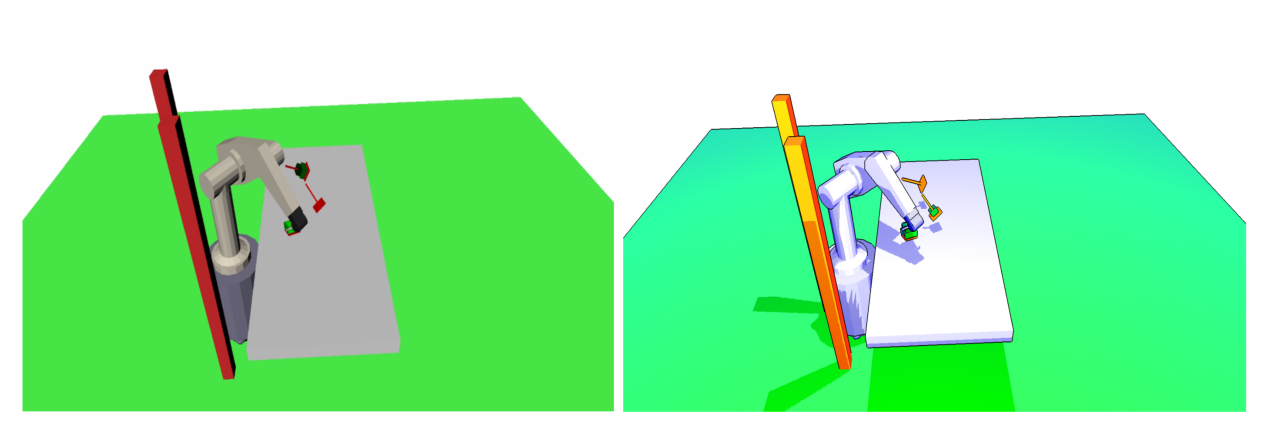
\includegraphics[scale=0.8]{beforeAfter_1.eps}
  \caption
{ \newline \hspace{\linewidth}
Figure showing original OpenRAVE simulation (left) and OpenRAVE simulation with Shady Robots' shaders implementation (right).}
  \label{fig:beforeafter}
\end{figure}

\subsection{End Project Survey}
Refer to next page for the survey that was used to determine if our implementations was able to improve confidence levels of users.

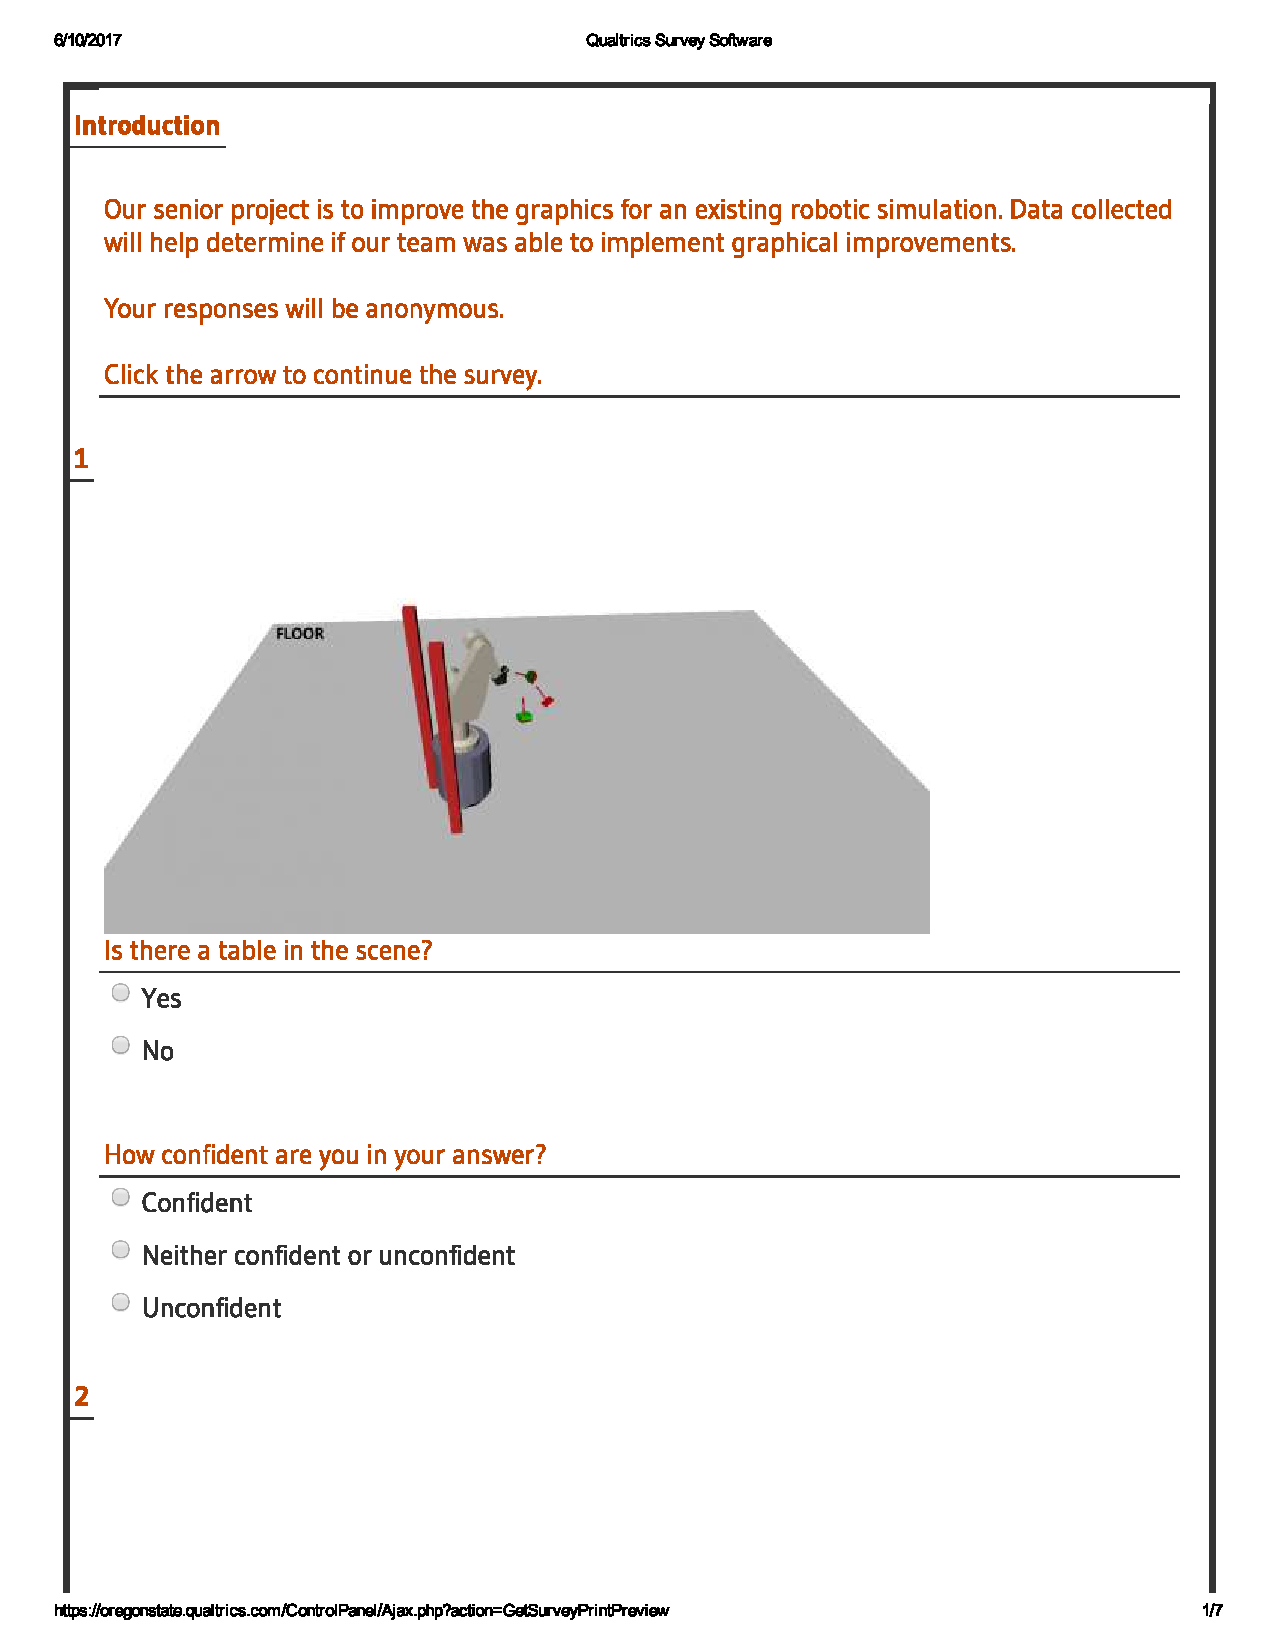
\includepdf[pages=-]{survey_example.pdf}


\end{flushleft}
\end{document}

